\documentclass[11pt]{report}
\usepackage{amsmath}
\usepackage{amssymb}
%\usepackage{bbm}
\usepackage{graphicx}
\usepackage{tikz}
\usepackage{longtable}
\usepackage{multirow}
\usepackage{array}
\usepackage{hhline}


\usetikzlibrary{tikzmark}

\newcommand{\linkV}[2]{%
	\begin{tikzpicture}[remember picture, overlay]
		\draw ([shift={(2mm, 6.6mm)}]{pic cs:#1}) to ([shift={(2mm, -2.8mm)}]{pic cs:#2});
	\end{tikzpicture}
}
\newcommand{\linkVV}[4]{%
	\begin{tikzpicture}[remember picture, overlay]
		\draw ([shift={(#3mm, 6.6mm)}]{pic cs:#1}) to ([shift={(#4mm, -2.8mm)}]{pic cs:#2});
	\end{tikzpicture}
}
\newcommand{\linkH}[2]{%
	\begin{tikzpicture}[remember picture, overlay]
		\draw ([shift={(-2mm, 2mm)}]{pic cs:#1}) to ([shift={(10mm, 2mm)}]{pic cs:#2});
	\end{tikzpicture}
}


\newcommand{\ubt}[1]{\textbf{\underline{#1}}}
\newcommand{\sps}{\\[0.2cm]}
\newcommand{\spn}[1]{\\[#1cm]}
\newcommand{\refn}[1]{(\ref{#1})}
\newcommand{\refx}[1]{\refn{eq:#1}}
\newcommand{\bt}[1]{\textbf{#1}}
\newcommand{\dsp}{\displaystyle}
\newcommand{\NI}{\noindent}
\newcommand{\real}{ \mathbb{R}}
\newcommand{\mbf}[1]{\mathbf{#1}}
\newcommand{\complex}{\mathbb{C}}
\newcommand{\sprime}{'}
\newcommand{\dprime}{''}
\newcommand{\tprime}{'''}
\newcommand{\sbracket}[1]{\left[#1\right]}
\newcommand{\example}[1]{\section*{\ubt{Example #1}}{~}\spn{-1}}
\newcommand{\examples}{\subsubsection*{Examples}{~}\spn{-1}}
\newcommand{\solution}{\subsubsection{\ubt{Solution}}{~}\spn{-1}}
\newcommand{\eg}{\subsection*{\ubt{Example}}{~}\spn{-1}}
%\newcommand{\real}{\mathbbm{R}}

\renewcommand{\baselinestretch}{1.5}
\renewcommand{\contentsname}{Table of Contents}
\renewcommand{\labelenumi}{\arabic{enumi})}
\renewcommand{\labelenumii}{\alph{enumii})}

%\setlength{\parindent}{1em}


\begin{document}
	
	%%%%%%%%%%%%%%%%%%%FRONT COVER%%%%%%%%%%%%%%%%%%%
	\addcontentsline{toc}{chapter}{TITLE PAGE}
	\clearpage
	\thispagestyle{empty}
	\begin{center}
		\Large \bt{ASSIGNMENT PROBLEM USING HUNGARIAN METHOD}
	\end{center}

	\hspace{7cm}
	
	\begin{center}
		\textbf{\textit{BY}}
	\end{center}
	
	\hspace{5cm}
	
	\begin{center}
		\large \textbf{EGUNJOBI, JESUJOBA DANIEL
			\\
			17/56EB048}
	\end{center}
	
	\hspace{9cm}
	
	\begin{center}
		A PROJECT SUBMITTED TO THE DEPARTMENT OF MATHEMATICS, FACULTY OF PHYSICAL SCIENCES, UNIVERSITY OF ILORIN, ILORIN, KWARA STATE, NIGERIA. 	IN PARTIAL FULFILLMENT OF REQUIREMENTS FOR THE AWARD OF BACHELOR OF SCIENCE (B. Sc.) DEGREE IN MATHEMATICS.
	\end{center}

	\hspace{7cm}
	
	\begin{center}
		\textbf{NOVEMBER, 2022}
	\end{center}

	\newpage
	\pagenumbering{roman}
	\addcontentsline{toc}{chapter}{CERTIFICATION}
	\section*{\begin{center}\textbf{\Large CERTIFICATION}   \end{center}}
	This is to certify that this project was carried out by \textbf{EGUNJOBI, Jesujoba Daniel} with Matriculation Number  17/56EB048 in the Department of Mathematics, Faculty of Physical Sciences, University of Ilorin, Ilorin, Nigeria, for the award of Bachelor of Science (B.Sc.) degree in Mathematics.
	\\
	\\
	................................... \qquad \qquad\qquad\qquad\qquad\qquad...................... \\
	Dr. Aderinto Yidiat \qquad\qquad\qquad\qquad\qquad\qquad\quad Date\\
	Supervisor\\
	\\
	\\
	\\
	...................................... \qquad\qquad\qquad\qquad\qquad\qquad ......................\\
	Prof. K. Rauf      \qquad\qquad\qquad\qquad\qquad\qquad\qquad\qquad\quad     Date\\
	Head of Department\\
	\\
	\\
	\\
	..................................... \qquad\qquad\qquad\qquad\qquad\qquad .......................\\
	Prof. T. O. Oluyo \quad\qquad\qquad\qquad\qquad\qquad\qquad\qquad         Date\\
	External Examiner 
	
	\newpage
	%%ACKNOLEDGMENTS%%
	\section*{\begin{center}\textbf{\Large ACKNOWLEDGMENTS}\end{center}}
	\addcontentsline{toc}{chapter}{ACKNOWLEDGMENTS} 					
	First and foremost, I want to give thanks and praises to Almighty God for His loving kindness and mercy for giving me the courage and determination to complete this research work.\\
	
	\NI My profound gratitude and appreciation goes to my supervisor Dr. Aderinto Yidiat for her useful and the valuable contribution, correction, and suggestion that greatly helps to the successful completion of this project.\\
	
	\NI My appreciation goes to my amiable and relentless Head of Department Prof. K. Rauf and my amiable Level Adviser, Dr. K.A. Bello for their words of encouragement, concern and support.\\
	
	\NI Also, my appreciation goes to all my esteem Lecturers: Prof. J. A. Gbadeyan, Prof. T. O. Opoola, Prof. O. M. Bamigbola, Prof. M. O. Ibrahim, Prof. O. A. Taiwo, Prof. R. B. Adeniyi, Prof. M. S. Dada, Prof. K. O. Babalola, Prof. A. S. Idowu, Prof. (Mrs) O. A. Fadipe-Joseph, Dr. E. O. Titiloye, Dr. (Mrs) Y. O. Aderinto, Dr (Mrs) C. N. Ejieji, Dr. B. M. Yisa, Dr. J. U. Abubakar, Dr. (Mrs) G. N. Bakare, Dr. (Mrs) I. F. Usamot, Dr. B. M. Ahmed, Dr. O. T. Olootu, Dr. O. A. Uwaheren, Dr. T. L. Oyekunle, Dr. O. Odetunde, Dr. A. Y. Ayinla and all other members of staff of the department of mathematics, who contributed greatly to my academic excellence, obtained during my period of study in the department. May God bless them all.\\
	
	\NI I am highly indebted to my loving and caring family especially my brother and sisters who have tersely contributed immensely toward the successful completion of my studies and academic activities.\\
	
	\NI To my friends inside and outside my department; big shout out to you all and thank you for your assistance and inputs during my course work and in this project. May our paths always be smooth and favour-filled. God bless you all.\\
	
	
	\newpage
	%%DEDICATION%%
	\section*{\begin{center}\textbf{\Large DEDICATION}\end{center}}
	\addcontentsline{toc}{chapter}{DEDICATION}
	This project work is dedicated to Almighty God who has brought me to this level in my undergraduate program. For His mercies, guidance and protection throughout my years of study.
	
	\newpage
	%%ABSTRACT%%
	\section*{\begin{center}\textbf{\Large ABSTRACT}\end{center}}
	\addcontentsline{toc}{chapter}{ABSTRACT}	
	\NI This project discusses the 
	
	\newpage
	%%%%%%%%%%%%%%%%%%%TABLE OF CONTENTS%%%%%%%%%%%%%%%%%%%
	\addcontentsline{toc}{chapter}{TABLE OF CONTENTS}
	\tableofcontents
	
	\newpage
	\pagenumbering{arabic}
	%%%%%%%%%%%%%%%%%%%CHAPTER ONE%%%%%%%%%%%%%%%%%%%
	\chapter{GENERAL INTRODUCTION}
	\section{Introduction}
	In today’s competitive word, having the right resources such as human and machines are important to the success of any institution or organisation and can be view like mechanical machines where the parts must fit and connect with each other for effective operation. These are highly-stakes tasks that requires careful consideration because being subjective and using only intuition in decision making can be detrimental to success and organizational growth. Manually creating a resources allocation and scheduling can be tedious and time-consuming because of many because of many computational procedures. There is need for local solutions that dynamically assign distinct agents to distinct tasks, while maximizing the total assignment benefit, hence the need for assignment problem. In this chapter, background of the study was presented together with the aims and objectives, scope and definitions of some basic terms.
	
	\section{Historical Background}
	Decision-making occurs in response to problems. It is a skill that is germane in today's competitive word. Therefore, having the right resources such as human and machines are important to the success of any institution or organisation and can be viewed as mechanical machines where the parts must fit and connect with each other correctly for effective operation. However, these are highly-stakes tasks that requires careful consideration, because being subjective and using only intuition in decision making can be detrimental to success and organizational growth. It may result in significant loss of value due to understaffing, under qualification or over qualification of assigned personnel, high turnover of poorly matched personnel and so on (Okrah, 2013). While the importance of decision-making is clear, dealing with pools of hundreds of tasks and resources result to an enormous amount of pressure and anxiety in making the right decisions rapidly, hence the need for optimization.\\
	
	\NI One important optimization technique is linear programming, which takes into consideration certain mathematical relationships in order to provide optimal practical solution to a problem. It can also be viewed as the application of algebra, in matrix form, in solving broad problems can be represented by linear equations. This exact method is used for planning and making decisions.\\
	
	\NI Linear programming helps us solve the complicated problem concerning allocation and scheduling of various resources such as men, machine, money, material, and time quantity satisfying certain constraints in the form of algebraically represented linear equations/inequalities so as to (Mallick, Bhoi, Jena, Sahoo, Humayn, \& Shahd 2021) It is applicable in various disciplines and fields such as business, commerce, marketing, industries and even education. Linear programming has many types of which assignment problem is part of it.\\
	
	\NI The assignment problem is a special type of linear programming problem and is one of the most studied, well-solved and important problems in combinatorial optimization with a plethora of practical applications (Aboudi \& Jornsten, 1990). It can proffer solutions that reveal insights on how to positively impact allocation and scheduling of tasks and improve efficiency. The assignment problem arises because available resources such as men, machines, etc. have varying degrees of efficiency for performing different tasks. Therefore, cost, profit or time of performing the different activities is different. Thus, the problem is how the assignments should be made so as to optimize the given objective (Gaglani, 2011). Basically, assignment problem can be a minimization or maximization model depending on the objective to be achieved. However, the
	basic objective of an assignment problem is to assign $n$ number of resources to $n$ number of activities so as to ensure that effectiveness is optimized. The assignment problem entails anticipating project allocation and scheduling in order to have the right people, with the right skill, at the right time, in the right place, at the right cost (Okrah, 2013).\\
	
	\NI In assignment problem, assignees are being assigned to perform tasks. It should be noted that assignees need not be people. They also could be machines, or vehicles, or plants, or even time slots to be assigned tasks. Exactly one resource has to be assigned to each of the distinct task in
	such way that maximum assignment benefit is achieved. Every assignment problem contains a matrix named cost or effectiveness matrix (Faudzi, Abdul-Rahman, \& Rahman, 2018). It may be noted that the assignment problem is a variation of the transportation problem with two characteristics (Akpan \& Abraham, 2016).
	
	\begin{enumerate}
		\item The cost matrix is a square matrix.
		\item The optimum solution for the problem would be such that there would be such that there would be only one assignment in a row or column of the cost matrix.
	\end{enumerate}
	
	\NI The assignment problem is important in the practical field. This problem has been commonly envisaged in many educational functions all over the world (Mim, Asadujjaman, \& Akter, 2022). With that, Faudzi, Abdul-Rahman and Rahman (2018) classified problems in educational domain into two, which are timetabling problem and allocation problem. The timetabling problem is further classified into examination, course, and school timetabling problems, while the allocation
	problem is divided into student-project allocation, new student allocation, and space allocation problems (Faudzi, Abdul-Rahman, \& Rahman, 2018).\\
	
	\NI In the educational domain, professors and doctors find themselves in a strife when matching and awarding prospective graduate students with research and teaching assistantship positions. Discriminating good matches from bad matches automatically is quite complex since hundreds of thousands of graduate students with thousands of skills are distributed in countries all over the world. Since there are no clear guidelines when matching an employee to a job, most times the
	professors rely on their intuition and instincts. Therefore, there is need to formulate a model that automates the discrimination of good matches from bad matches. The research is of paramount importance as it seeks to find the optimal assignment of students-assistantship allocation that will
	helps in promoting teaching-learning processes, thereby improving the educational quality and national development in general.
	
	\section{Definitions of some Basic Terms}
	\subsection{Assignment Problem}
	A basic combinatorial optimization problem is the assignment problem. This is special types of linear programming problem which deals with the allocation of various
	resources to various objects where the cost is minimized.
	
	\subsection{Combinatorial Optimization}
	In mathematics, the term combinatorial is used to describe a type of problem which deals with problems with minimizing and maximizing a function of variables subject to inequality or equality constraints and restrictions on all or some of the restrictions.
	
	\subsection{Optimal Solution}
	A feasible solution (not necessarily basic) is said to be optimal if it minimizes
	the total cost.
	
	\section{Aim and Objectives of the Study}
	Therefore, the broad aim of this research is to determine the optimal assignment (allocation) schedule of five teaching assistantship positions to five different prospective students, on one-toone basis. By applying the Hungarian method and determining the best way of allocating students assistantship positions, it will, to a large extent enhance the number of mathematical assistantships and scholarships in the future.
	
	\section{Scope of the Study}
	The scope of the study is to focus on how teaching assistantship positions are assigned to prospective graduate students to handle the courses so as to minimize the total course scheduling and preparatory time and ensure that effectiveness is optimized. It is assumed that all the graduate students that applied for the positions are competent enough to deliver satisfactorily.
	
		
	%%%%%%%%%%%%%%%%%%%CHAPTER TWO%%%%%%%%%%%%%%%%%%%
	\chapter{LITERATURE REVIEW}
	\section{Introduction}
	In this chapter, the related work done by researchers so far in the area of assignment problem and how they have been solved till date were discussed. Likewise, the researcher also seek to understand the mathematical formulations, types, classification and methods solving assignment problem through a review of books and journals which are directly related to the topic of study.
	
	\section{Mathematical Formulation of Assignment Problem}
	The standard assignment problem requires that there be as many resources to tasks, say n of each. In this case, there are exactly $n!$ different ways to assign the tasks to the resources on a one-to-one basis. This follows because there are $n$ ways to assign the first task, $n-1$ ways to assign the second, $n-2$ ways to assign the third, and so on, with a total of $n \cdot (n-1) \cdot (n-2) \cdots 3 \cdot 2 \cdot 1 = n!$ possible assignments. Among these $n!$ possible assignments, the optimal assignment can now be solved for.
	(Odior, Charles-Owaba, \& Oyawale, 2010).\\
	
	\NI Therefore, a linear model in standard form for the assignment problem can be expressed mathematically as follow:
	\begin{eqnarray}
		\text{Minimize } Z = \sum_{i=1}^{n}\sum_{j=1}^{n}c_{ij}x_{ij}
	\end{eqnarray}
	subject to the constraints
	\begin{eqnarray}
		\sum_{j=1}^{n}x_{ij} &=& 1 ~~~\forall ~~i ~~~\text{(resource availability)}\sps
		\sum_{i=1}^{n}x_{ij} &=& 1 ~~~\forall ~~j ~~~\text{(activity requirement)}
	\end{eqnarray}
	and $x_{ij} = 0$ or $1$ , for all $i$ and $j$ where $c_{ij}$ represents the cost of assignment of resource $i$ to activity $j$.\\
	
	\NI This mathematical model of assignment problem is a particular case of the transportation
	problem for two reasons: 
	\begin{enumerate}
		\renewcommand{\labelenumi}{(\roman{enumi})}
		\item the cost matrix is a square matrix, and
		\item the optimal solution table (matrix) for the problem would have only one assignment in a given row or a column.
	\end{enumerate}
	
	\begin{figure}[!h]
		\centering
		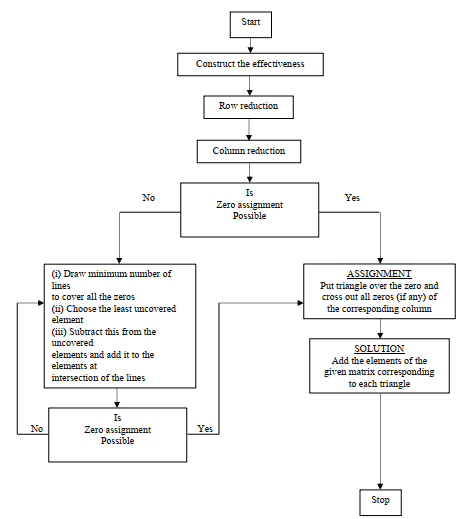
\includegraphics[width=1.02\linewidth]{mt}
		\caption{Flow chart for Assignment problem}
	\end{figure}
	\newpage
	\section{Types of Assignment Problem}
	The relevant data for any assignment problem can be summarized in a matrix format using a tableau called the assignment costs or effectiveness tableau. The two types of assignment problem as described as follows:
	
	\subsection{Balanced Assignment Problem}
	The assignment problem is to be balanced if the cost or effectiveness matrix has equal number of rows and columns or equivalently, if the given problem is a square matrix (i.e. $n\times n$ matrix)(Kabiru, Saidu, Abdul, \& Ali, 2017).
	
	\subsection{Unbalanced Assignment Problem}
	Any assignment problem is said to be unbalanced if the cost or effectiveness matrix is not a square matrix, i.e. the no of rows and the no of columns are not equal. In order to balance it, we can always add as many dummy origins or dummy destinations as necessary. The assignment costs of the dummy origins or dummy destinations are zero.
	
	\section{Classification of Assignment Problem in Educational Domain}
	Assignment problem is commonly encountered in educational settings all over the world. Within the education domain, Faudzi, Abdul-Rahman and Rahman (2018) classified the assignment problem into two namely: timetabling problem and allocation problem. The timetabling problem is further classified into examination, course, and school timetabling problems, while the allocation problem is divided into student-project allocation, new student allocation, and space allocation problems. The all these problems are discussed below:
	
	\subsection{Timetabling Problem}
	Timetabling problem is considered as an assignment problem. A timetable usually provides information about the time for particular events to occur and eventually relates to the resources allocation (Wren, 1996). Besides, timetabling is described as an assignment of events to a limited number of timeslots and rooms subject to prescribed constraints (Lu \& Hao, 2008). In reality, allocation of resources at a specified time is indeed necessary. The problem is challenging because one has to schedule a large number of entities and satisfy a number of constraints and preferences. Furthermore, timetabling problem is classified into three subproblems, which are examination timetabling problem (ETP), course timetabling problem (CTP), and school timetabling problem (STP). They are further discussed in the following subsections.
	
	\subsubsection{Examination Timetabling Problem}
	The examination timetabling problem (ETP) is defined as an assignment of a set of examinations to a set of timeslots while simultaneously satisfying several problem constraints. According to Carter and Laporte (1996), ETP is defined as a process of assigning examinations to a limited number of timeslots with the aim of producing high quality timetable subject to constraints.
	
	\subsubsection{Course Timetabling Problem}
	Course timetabling refers to the process of assigning courses, rooms, students, and lecturers to a fixed time period, typically a working week, while satisfying a given set of constraints (Cote, Wong, \& Sabourin, 2010).According to Obit (2010), university course timetabling is considered
	as a weekly schedule of all university lecturers to a set of courses and at the same time to prevent the lecturers to have students in common at two different timeslots.
	
	\subsubsection{School Timetabling Problem}
	The school timetabling problem (STP) is about generating school timetable that usually follows a cycle every week for all classes, in which the objective is to avoid teachers from attending two classes at the same time. In school timetabling, students are normally pre-assigned, while only teachers and rooms need to be assigned in the timetabling problem. As such, Cerdeira-Pena et al. (2008) stated that STP is aimed at assigning period for teacher to certain subject in a specified group by considering groups of students and teachers in a fixed period scheduling.
	
	\subsection{Allocation Problem}
	Allocation problem is considered a assignment problem. In fact, the allocation problem has been cited widely as a fundamental combinatorial optimization problem under optimization or operation research branch. The allocation problem is a famous problem discussed in the literature with
	various types of applications, including the education domain. This problem is categorised into three subproblems, which are student-project allocation problem (SPAP), new student allocation problem (NSAP), and space allocation problem (SAP). They are further discussed in the following
	subsections.
	
	\subsubsection{Student-Project Allocation Problem}
	The student-project allocation problem (SPAP) is related to assigning a person to a particular project or cases based on preference or interest of student and lecturer (Wren, 1996). SPAP includes a set of projects, students, and lecturers, whereby every unique lecturer is offered a project and both the lecturers and projects have some capacity constraints.
	
	\subsubsection{New Student Allocation Problem}
	The new student allocation problem (NSAP) is a clustering problem in allocating new students to their corresponding class with minimum intelligence gap by sorting method: a group of new students with similar ranking and assigned into the same class.
	
	\subsubsection{Space Allocation Problem}
	The space allocation problem (SAP) refers to a problem to allocate resources to space areas, for example, allocating rooms and at the same time satisfying several requirements and constraints. Likewise, Burke and Varley (1997) described SAP as an allocation of rooms or areas of space for detailed function.
	
	\section{Method of solving Assignment Problem}
	So far in the literature, there are mainly four solution methods so called complete enumeration method, simplex method, transportation method and Hungarian method for solving Assignment Problem. They are further discussed in the following subsections.
	
	\subsection{Enumeration method}
	In this method, a list of all possible assignments among the given resources (like men, machines, etc.) and activities (like jobs, sales areas, etc.) is prepared. Then an assignment involving the minimum cost (or maximum profit), time or distance is selected. If two or more assignments have
	the same minimum cost (or maximum profit), time or distance, the problem has multiple optimal solutions. In general, if an assignment problem involves $n$ resources/tasks, then there are in total $n!$ possible assignments. However, when $n$ is large, the method is unsuitable for manual calculations. Hence, this method is suitable only for small $n$.
	
	\subsection{Simplex Method}
	Since each assignment problem can be formulated as a 0 or 1 which becomes integer linear programming problem. Such a problem can be solved by the simplex method also. As can be seen in the general mathematical formulation of the assignment problem, there are $n\times n$ decision variables and $n+n$ or $2n$ equalities. However, it is, difficult to solve manually.
	
	\subsection{Transportation Method}
	Since an assignment problem is a special case of the transportation problem, it can also be solved
	by transportation methods. However, every basic feasible solution of a general assignment problem having a square payoff matrix of order n should have more$ m+n-1= n+n-1=2n-1$
	assignments. But due to the special structure of this problem, any solution cannot have more than $n$ assignments. Thus, the assignment problem is inherently degenerate. In order to remove degeneracy, $(n-1)$ number of dummy allocations will be required in order to proceed with the
	transportation method. Thus, the problem of degeneracy at each solution makes the transportation method computationally inefficient for solving an assignment problem.
	
	\subsection{Hungarian Method}
	Assignment problems can be formulated with techniques of linear programming and transportation problems. As it has a special structure, it is solved by the special method called Hungarian method. This method was developed by D. Konig, a Hungarian mathematician and is therefore known as the Hungarian method of assignment problem. In order to use this method, one needs to know only the cost of making all the possible assignments. Each assignment problem has a matrix (table) associated with it. Normally, the objects (or people) one wishes to assign are expressed in rows, whereas the columns represent the tasks (or things) assigned to them. The number in the table would then be the costs associated with each particular assignment. Hungarian method is based on the principle that if a constant is added to the elements of cost or effectiveness matrix, the optimum solution of the assignment problem is the same as the original problem. Original cost or effectiveness matrix is reduced to another cost or effectiveness matrix by adding a constant value
	to the elements of rows and columns of cost or effectiveness matrix where the total completion time or total cost of an assignment is zero. This assignment is also referred as the optimum solution since the optimum solution remains unchanged after the reduction. Hungarian method is one of the best available for solving an assignment problem.
	
	\section{Review on Assignment Problem}
	Mim, Asadujjaman and Akter (2022) presented a new branch and bound algorithm for solving the assignment problems that uses a lower bound based with branching procedure. This is special type of linear programming problem dealing with the allocation of various resources to the various activities on one to one basis. This mathematical based model is suggested to assign the agents to the organization or firm where the established Hungarian method have not been used but we use both row and column operation. After both row and column operation with branch and bound technique followed by integer programming the researcher got the same optimal value as found by the established Hungarian method. The proposed solution algorithm was simple but the implementation of these agents allocation problem in firm was time consuming.\\
	
	\NI Al-Zubaydi (2020) compared a new approach and the Hungarian method to solve assignment problem. The researcher converted an assignment into a complete bipartite graph using Kruskal's Algorithm in order to find the minimum spanning tree, and obtaining the most optimal assignment. Thus the most optimal assignment was found. The 2 results of various cases were compared Hungarian algorithm, and the results were satisfying in both methods. The researcher also mentioned that accessing the most optimal assignment by employing those two methods is easy however the method Kruscal's algorithm was easiest to have optimal solution.\\
	
	\NI Solaja, Abiodun, Ekpudu, Abioro and Akinbola (2019) applies the assignment model to the course allocation problem in Nigeria tertiary institution in order to maximize lecturers’ effectiveness. A well-structured questionnaire was used to obtain data from lecturers and solved with Hungarian
	method. Courses available for final year students are derived from the 2018/2019 university first semester timetable. Out of six (6) courses that students are to be taken in the semester, four (4) are core courses that are mandatory for students in the department while other two (2) courses are elective. The study revealed that adoption of the assignment model in course allocation will help the institution to experience 13.20\% increment in lecturers’ effectiveness in taking each topic in analysis for business decision. This will lead to increase in the quality of education students get. The study concluded that assignment model is a unique model that can be used to solve course allocation problems in tertiary institutions.\\
	
	\NI The Quadratic assignment problem (QAP) is a simplest form concerned with locating facilities on locations, such that total transportation costs are minimized. Ahyaningsih (2017) proposed a Combined Strategy (random point strategy to get initial starting point and then use forward exchange strategy and backward exchange strategy to get ‘optimal’ solution) for Solving Quadratic Assignment Problem. The researcher used QAPLIB for computational experience and the combined strategy was able to solve problem instance Esc 16b, Esc 16c, and Esc 16h in relatively short computing time. Based on the experiment for problem instances Esc 16b, Esc 16c, and Esc
	16h, optimum value was reached at iteration 500. Finally, the researcher presented a comparative study between Combined Strategy and Data –Guided Lexisearch Algorithm. The computational study shows the effectiveness of the proposed combined strategy.\\
	
	\NI Kabiru, Saidu, Abdul andAli (2017) utilized assignment model in assigning teachers to science subjects in Nigeria. The model was solved with the help of Hungarian method and LINGO. The study covers data gathered from the period of two academic sessions (2014/15-2015/16). The head of the staff has the problem of allocating teachers to five different subjects which includes: Mathematics, English, Physics, Chemistry and Biology offered by science class in his school. He has availability of five staffs named A, B, C, D, and E graduates teachers who have handled or taught at least one of these subjects in the past two academic sessions and have been evaluated with a score from 0 to 100 (Basic rating = 100) regarding the ability of each staff to each subject
	respectively. The results from both methods yielded the same optimal outcome. It reveals that the total minimum opportunity that will maximize the educational quality is 84 and the total maximum effectiveness that will maximize the educational quality is 416. However, the two techniques
	produced the same result.\\
	
	\NI Baumelt et al. (2016) developed a parallel assignment problem solving algorithm allowing the Nurse ReRostering Problem (NRRP) to be (partially) solved on a graphics processing unit (GPU). In the core, the algorithm is a constructive algorithm inspired by Moz and Pato’s work. The authors created both a homogeneous and a heterogeneous version of the parallel algorithm – in the homogeneous version the algorithm is run solely on the graphic processing unit and in the heterogeneous version of the algorithm the problem is solved partially on the GPU and partially
	on the central processing unit (CPU). To explore the effectiveness of the parallel approach, the authors compared both models to a sequential version of the algorithm. Test were done using the benchmark instances made available by Moz and Pato. All algorithms returned solutions of comparable quality as achieved with Moz and Pato’s genetic algorithm. As for the computation times, the homogeneous algorithm performed the best, yielding a 12 times speed up compared to the sequential algorithm. The homogeneous algorithm was able to find solutions for all instances in a matter of seconds. Although the speed up achieved by using a parallel algorithm
	on a GPU is promising, the authors do point out some limitations of the method. Mainly, the design of the algorithm must be suited for the architecture. For instance, to achieve speedup, branch divergence should be avoided in the code as much as possible. Nonetheless, the authors show a
	promising new approach for solving the NRRP.\\
	
	\NI Thongsanit (2014) developed mathematical model and design methods to solve the problem. The assignment problem uses the information from the Faculty of Engineering and Industrial
	Technology at Silpakorn University in the first semester, 2012. Excel’s Premium Solver is applied in this study. It was found that Excel’s Premium Solver can solve this classroom allocation problem with the process time in seconds. The total cost was reduced 27,920 baht / semester. The solution
	from the model was compared to the solution from the practical use or the manual assignment with total 115 courses (all courses from Monday to Friday). The solutions from the manual assignment are investigated. It was found that some solutions violated the constraints in the model.\\
	
	\NI Toroslu and Arslanoglu (2012), presented variations of the standard assignment problem with matching constraints by introducing structures in the partitions of the bipartite graph, and by defining constraints on these structures. According to the first constraint, the matching between
	the two partitions should respect the hierarchical-ordering constraints defined by forest and level graph structures produced by using the nodes of the two partitions respectively. In order to define the second constraint, the nodes of the partitions of the bipartite graph are distributed into mutually exclusive sets. The set-restriction constraint enforces the rule that in one of the partitions all the elements of each set should be matched with the elements of a set in the other partition. Even with one of these constraints the assignment problem becomes an NP-hard problem. The extended assignment problem with both the hierarchical-ordering and set-restriction constraints becomes an NP-hard multi-objective optimization problem with three conflicting objectives; namely, minimizing the numbers of hierarchical-ordering and set-restriction violations, and maximizing the summation of the weights of the edges of the matching. Genetic algorithms are proven to be very successful for NP-hard multi-objective optimization problems. The authors also proposed genetic algorithm solutions for different versions of the assignment problem with multiple objectives based on hierarchical and set constraints, and empirically showed the performance of these solutions.\\
	
	\NI Sanei et al., (2011) studied the problem of space assignment for the products in a warehouse considering various operational constraints. These constraints are mainly set to prevent decentralization of products in storage locations considering more explicit and more exquisite
	inventory control. A linear integer programming model and a heuristic algorithm based on the branch and bound method is proposed to solve the problem. Further, software has been developed based on proposed algorithm for industrial usage. An experimental study, based on real data from an auto-industry shows the efficiency of the proposed algorithm achieving reasonable solutions.\\
	The channel-assignment problem is important in mobile telephone communication. Since the usable range of the frequency spectrum is limited, the optimal channel-assignment problem has become increasingly important. Omid (2010) presented a model and the goal of this is to find a
	channel assignment to requested calls with the minimum number of channels subject to interference constraints between channels. This algorithm consists of: 
	\begin{enumerate}
		\renewcommand{\labelenumi}{(\roman{enumi})}
		\item the fixed channel assignment stage;
		\item the neural network stage. In the first stage, the calls in a cell determining the lower bound on the total number of channels are assigned channels at regular intervals; then the calls in adjacent six cells are assigned channels by a cluster heuristic method sequentially.
	\end{enumerate}
	 In the second stage, the calls in the remaining cells are assigned channels by a binary neural network. The performance is verified through solving well-known benchmark problems.\\
	 
	\NI Mingfang (2010) studied the weapon-target assignment (WTA) problem which has wide applications in the area of defense-related operations research. This problem calls for finding a proper assignment of weapons to targets such that the total expected damaged value of the targets to be maximized. The WTA problem can be formulated as a nonlinear integer programming problem which is known to be NP-complete. There does not exist any exact method for the WTA
	problem even small size problems, although several heuristic methods have been proposed. In this paper, Lagrange relaxation method is proposed for the WTA problem. The method is an iterative approach which is to decompose the Lagrange relaxation into two sub-problems, and each subproblem can be easy to solve to optimality based on its specific features.\\
	
	\NI Nagarajan and Solairaju (2010) presented studies which $a_{ij}$ was considered to be trapezoidal and triangular numbers denoted by $a_{ij}$ which are more realistic and general in nature. Robust‘s ranking method has been used for ranking the fuzzy numbers. The fuzzy assignment problem has been transformed into crisp assignment problem in the linear programming problem form and solved by using Hungarian method; Numerical examples show that the fuzzy ranking method offers an effective tool for handling the fuzzy assignment problem.\\
	
	\NI Wang and Liu (2010) presented a new algorithm on a special assignment problem in which the real assigned jobs are less than or equal to both the total persons and the total jobs. To this special assignment problem the authors posed the concept of reserve point, discussed the character of
	reserve point and accessed to relevant conclusion a new method to solve this special assignment problem is given through increasing reserve points finally.\\
	
	\NI Bettina and Alexandru (2009) presented a similar approach to one-sided assignment problems as Sasaki (1995) for two-sided assignment problems. The authors showed that for the class of solvable one-sided assignment problems (i.e., the subset of one-sided assignment problems with a
	non-empty core), if a sub-solution of the core satisfies (indifference with respect to dummy agents, continuity, and consistency) or (Pareto indifference and consistency), then it coincides with the core. However, the authors also prove that on the class of all one-sided assignment problems
	(solvable or not), no solution satisfies consistency and coincides with the core whenever the core is non-empty. Finally, the authors commented on the difficulty in obtaining further positive results for the class of solvable one-sided assignment problems in line with Sasaki's (1995) characterizations of the core for two-sided assignment problems.\\
	
	\NI Semih, Umut and Bilgehan (2008) presented a distribution-type warehouse assignment problem that various types of products were collected from different suppliers for storing in the warehouse for a determined period and for delivery to different customers. The aim of their study was to
	design a multiple-level warehouse shelf configuration which minimized the annual carrying costs. Since proposed mathematical model was shown to be NP-hard, a Particle Swarm Optimization algorithm (PSO) as a novel heuristic was developed for determining the optimal layout.\\
	
	\NI Naveh, Richter, Gresh, Altshuler and Connors (2007) presented a novel solution designed to bridge the gap between the need for high-quality matches and the need for timeliness. By applying constraint programming, a subfield of artificial intelligence, the authors dealt successfully with the complex constraints encountered in the field and reach near-optimal assignments that take into account all resources and positions in the pool. The considerations include constraints on job role, skill level, geographical location, language, potential retraining, and many more. Constraints were applied at both the individual and team levels. The authors introduced a technology and then describe its use by IBM Global Services, where large numbers of service and consulting employees are considered when forming teams assigned to customer projects.\\
	
	\NI Katta and Jay (2005) presented the problem of allocating a set of indivisible objects to agents in a fair and efficient manner. In a recent paper, Bogomolnaia and Moulin (2001) considered the case in which all agents have strict preferences, and proposed the Probabilistic Serial (PS) mechanism; they define a new notion of efficiency, called ordinal efficiency, and prove that the probabilistic serial mechanism finds an envy-free ordinarily efficient assignment. However, the restrictive assumption of strict preferences is critical to their algorithm. The author’s main contribution was an analogous algorithm for the full preference domain in which agents are allowed to be indifferent between objects. The author’s algorithm was based on a reinterpretation of the PS mechanism as an iterative algorithm to compute a flow in an associated network. In addition the authors showed that on the full preference domain it is impossible for even a weak strategy proof mechanism to find a random assignment that is both ordinarily efficient and envy-free.\\
	
	\NI Zhang and Jonathan (2002) studied a multi-period assignment problem that arises as part of a weekly planning problem at mail processing and distribution centers. These facilities contain a wide variety of automation equipment that is used to cancel, sort, and sequence the mail. The input
	to the problem is an equipment schedule that indicates the number of machines required for each job or operation during the day. This result is then post-processed by solving a multi-period assignment problem to determine the sequence of operations for each machine. Two criteria are
	used for this purpose. The first is to minimize the number of startups, and the second is to minimize the number of machines used per operation. The problem is modeled as a 0–1 integer program that can be solved in polynomial time when only the first criterion is considered. To find solutions in
	general, a two-stage heuristic is developed that always obtains the minimum number of startups, but not necessarily the minimum number of machines per operation. In a comparative study, high quality solutions were routinely provided by the heuristic in negligible time when compared to a commercial branch-and-bound code (Xpress). For most hard instances, the branch-and-bound code was not able to even find continuous solutions within acceptable time limits.\\
	
	\NI Anshuman and Rudrajit (2006) solved the generalized ―Assignment problem through genetic algorithm and simulated annealing. The generalized assignment problem is basically the ―N menN jobs problem where a single job can be assigned to only one person in such a way that the overall cost of assignment is minimized. While solving this problem through Genetic Algorithm (GA), a unique encoding scheme is used together with Partially Matched Crossover (PMX). The
	population size can also be varied in each iteration. In Simulated Annealing (SA) method, an exponential cooling schedule based on Newtonian cooling process is employed and
	experimentation is done on choosing the number of iterations (m) at each step. The source codes for the above have been developed in C language and compiled in GCC. Several test cases have been taken and the results obtained from both the methods have been tabulated and compared against the results obtained by coding in AMPL.\\
	
	\NI Nuass (2003) described a special purpose branch-and-bound algorithm that utilizes linear programming cuts, feasible-solution generators, Lagrangean relaxation, and sub-gradient optimization. The author presented computational results for solving "hard" problems with up to 3,000 binary variables. An unanticipated benefit of the algorithm is its ability to generate good feasible solutions early in the process whose solution quality generally dominates the solutions generated by two recently published heuristics. Furthermore, the computation time required is often less than the time taken by the heuristics. Thus, the authors have an optimizing algorithm that can be used quite effectively as a heuristic when proof of optimality is not an absolute
	requirement.\\
	
	\NI Franses and Gerhard (2003) studied an assignment problem particular to the personnel scheduling of organisations such as laboratories. Here the authors have to assign tasks to employees. The authors focused on the situation where this assignment problem reduces to constructing maximal matchings in a set of interrelated bipartite graphs. The authors described in detail how the continuity of tasks over the week is achieved to suit the wishes of the planner. Finally the authors discussed the implementation of the algorithm in the package IPS. Its main characteristic is the introduction of profiles, which easily allows the user to steer the algorithm.
	

	%%%%%%%%%%%%%%%%%%%CHAPTER THREE%%%%%%%%%%%%%%%%%%%
	\chapter{METHODOLOGY}
	\section{Introduction}
	In this chapter, the researcher presented the Hungarian method for solving the Assignment Problem in this study.
	
	\section{Hungarian Method: Algorithm}
	\begin{enumerate}
		\renewcommand{\labelenumi}{\bt{Step \arabic{enumi}:}}
		\item Prepare row reduced matrix by selecting the minimum values for each row and subtracting it from other elements of the row.
		\item Prepare column reduced matrix by subtracting minimum value of the column from the other values of that column.
		\item Check the row and box the first zero and cross out the other zeros in the column and row.
		\item Apply the optimal test: if each row and column contain one exactly encircled zero, then the current assignment is optimal. However, if one row or column is without an assignment, then	the assignment is not optimal.
		\item Tick all unassigned rows. If a ticked row has a zero or more, then tick the corresponding column. If a ticked column has an assignment, then tick the corresponding row.
		\item Draw a line each through unticked rows. Also, draw a line through the ticked column to form an intersection.
		\item Determine the smallest cost element not covered by the straight line. Subtract this smallest cost element from all the uncovered elements and add this to all those elements which are lying in	the intersection of these straight lines and do not change the remaining element which lie on the straight lines.
		\item Repeat steps 3, 4, 5 6 and 7, until an optimum assignment is obtained.
	\end{enumerate}
	
	\section{Worked Examples}
	\example{3.1}
	A pharmaceutical company producing a single product sold it through five agencies situated in different cities. All of a sudden, there rouse a demand for the product in another five cities that didn’t any agency of the company. The company is now facing the problem of deciding on how to assign the existing agencies in order to dispatch the product to needy cities in such a way that the travelling distance is minimized. The distance between the surplus and deficit cities
	(in km) is given in the following table.
	\begin{longtable}{|c|>{\centering\arraybackslash}m{1.2cm}|>{\centering\arraybackslash}m{1.15cm}|>{\centering\arraybackslash}m{1.15cm}|>{\centering\arraybackslash}m{1.15cm}|>{\centering\arraybackslash}m{1.15cm}|>{\centering\arraybackslash}m{1.15cm}|}
		\hline
		\multicolumn{7}{|c|}{\bt{Deficit cities}}\\\hline
		\multirow{6}{*}{Surplus Cities} & & \bt{a} & \bt{b} & \bt{c} & \bt{d} & \bt{e}\\\cline{2-7}
		& \bt{A}& 160 & 130 & 115 & 190 & 200\\\cline{2-7}
		& \bt{B} & 135 & 120 & 130 & 160 & 175\\\cline{2-7}
		& \bt{C} & 140 & 110 & 125 & 170 & 185\\\cline{2-7}
		& \bt{D} & 50 & 50 & 80 & 80 & 110\\\cline{2-7}
		& \bt{E} & 55 & 35 & 80 & 80 & 105\\\hline
	\end{longtable}
	\NI Determine the optimum travelling distance.
	\solution
	\begin{enumerate}
		\renewcommand{\labelenumi}{\bt{Step \arabic{enumi}:}}
		\item Prepare row reduced matrix by selecting the minimum values for each row and subtracting it from other elements of the row.
		\begin{longtable}{|>{\centering\arraybackslash}m{1.4cm}|>{\centering\arraybackslash}m{1.4cm}|>{\centering\arraybackslash}m{1.4cm}|>{\centering\arraybackslash}m{1.4cm}|>{\centering\arraybackslash}m{1.4cm}|>{\centering\arraybackslash}m{1.4cm}|}
			\hline
			 & \bt{a} & \bt{b} & \bt{c} & \bt{d} & \bt{e}\\\hline
			\bt{A}& 45 &15& 0& 75& 85\\\hline
			\bt{B} & 15 &0& 10& 40 &55\\\hline
			 \bt{C} & 30 &0 &15 &60 &75\\\hline
			\bt{D} & 0 &0& 30& 30& 60\\\hline
			\bt{E} & 20 &0 &45& 45 &70\\\hline
		\end{longtable}
		%%%%%%%%%
		\item Prepare column reduced matrix by subtracting minimum value of the column from the other values of that column
		\newpage
		\begin{longtable}{|>{\centering\arraybackslash}m{1.4cm}|>{\centering\arraybackslash}m{1.4cm}|>{\centering\arraybackslash}m{1.4cm}|>{\centering\arraybackslash}m{1.4cm}|>{\centering\arraybackslash}m{1.4cm}|>{\centering\arraybackslash}m{1.4cm}|}
			\hline
			& \bt{a} & \bt{b} & \bt{c} & \bt{d} & \bt{e}\\\hline
			\bt{A}& 45 &15& 0& 45& 30\\\hline
			\bt{B} & 15 &0& 10& 10 &0\\\hline
			\bt{C} & 30 &0 &15 &30 &20\\\hline
			\bt{D} & 0 &0& 30& 0& 5\\\hline
			\bt{E} & 20 &0 &45& 15 &15\\\hline
		\end{longtable}
		%%%%%%%%%
		\item Check the row and box the first zero and cross out the other zeros in the column and row.
		\begin{longtable}{|>{\centering\arraybackslash}m{1.4cm}|>{\centering\arraybackslash}m{1.4cm}|>{\centering\arraybackslash}m{1.4cm}|>{\centering\arraybackslash}m{1.4cm}|>{\centering\arraybackslash}m{1.4cm}|>{\centering\arraybackslash}m{1.4cm}|}
			\hline
			& \bt{a} & \bt{b} & \bt{c} & \bt{d} & \bt{e}\\\hline
			\bt{A}& 45 &15& [0]& 45& 30\\\hline
			\bt{B} & 15 &$\times$& 10& 10 &[0]\\\hline
			\bt{C} & 30 &[0] &15 &30 &20\\\hline
			\bt{D} & [0] &$\times$& 30& $\times$& 5\\\hline
			\bt{E} & 20 &$\times$ &45& 15 &15\\\hline
		\end{longtable}
		%%%%%%%%%
		\item Apply the optimal test: if each row and column contain one exactly encircled zero, then the current assignment is optimal. However, if one row or column is without an assignment, then the assignment is not optimal.
		\\ Since each row and column does not contain exactly one encircled zero, then the current is not
		optimal and we proceed to the next step.
		\item Tick all unassigned rows. If a ticked row has a zero or more, then tick the corresponding column. If a ticked column has an assignment, then tick the corresponding row.
		\begin{longtable}{|>{\centering\arraybackslash}m{1.4cm}|>{\centering\arraybackslash}m{1.4cm}|>{\centering\arraybackslash}m{1.4cm}|>{\centering\arraybackslash}m{1.4cm}|>{\centering\arraybackslash}m{1.4cm}|>{\centering\arraybackslash}m{1.4cm}|>{\centering\arraybackslash}m{1.4cm}|}
			\hline
			& \bt{a} & \bt{b} & \bt{c} & \bt{d} & \bt{e}&\\\hline
			\bt{A}& 45 &15& [0]& 45& 30&\\\hline
			\bt{B} & 15 &0& 10& 10 &[0]&\\\hline
			\bt{C} & 30 &[0] &15 &30 &20&$\checkmark$\\\hline
			\bt{D} & [0] &0& 30& 0& 5&\\\hline
			\bt{E} & 20 &0&45& 15 &15& $\checkmark$\\\hline
			& & $\checkmark$ & & & &\\\hline
		\end{longtable}
		%%%%%%%%%
		\item Draw a line each through unticked rows. Also, draw a line through the ticked column to form an intersection.
		\begin{longtable}{|>{\centering\arraybackslash}m{1.4cm}|>{\centering\arraybackslash}m{1.4cm}|>{\centering\arraybackslash}m{1.4cm}|>{\centering\arraybackslash}m{1.4cm}|>{\centering\arraybackslash}m{1.4cm}|>{\centering\arraybackslash}m{1.4cm}|>{\centering\arraybackslash}m{1.4cm}|}
			\hline
			& \bt{a} & \bt{b} & \bt{c} & \bt{d} & \bt{e}&\\\hline
			\bt{A}& \tikzmark{a1}45 &\tikzmark{d1}15& [0]& 45& \tikzmark{a2}30&\\\hline
			\bt{B} & \tikzmark{b1}15 &0& 10& 10 &\tikzmark{b2}[0]&\\\hline
			\bt{C} & 30 &[0] &15 &30 &20&$\checkmark$\\\hline
			\bt{D} & \tikzmark{c1}[0] &0& 30& 0& \tikzmark{c2}5&\\\hline
			\bt{E} & 20 &\tikzmark{d2}0&45& 15 &15& $\checkmark$\\\hline
			& & $\checkmark$ & & & &\\\hline
		\end{longtable}
		\linkH{a1}{a2}\linkH{b1}{b2}\linkH{c1}{c2}\linkV{d1}{d2}
		%%%%%%%%%
		\item Determine the smallest cost element not covered by the straight line. Subtract this smallest cost element from all the uncovered elements and add this to all those elements which are lying in the intersection of these straight lines and do not change the remaining element which lie on the straight lines.
		\begin{longtable}{|>{\centering\arraybackslash}m{1.4cm}|>{\centering\arraybackslash}m{1.4cm}|>{\centering\arraybackslash}m{1.4cm}|>{\centering\arraybackslash}m{1.4cm}|>{\centering\arraybackslash}m{1.4cm}|>{\centering\arraybackslash}m{1.4cm}|}
			\hline
			& \bt{a} & \bt{b} & \bt{c} & \bt{d} & \bt{e}\\\hline
			\bt{A}& 45 &30& 0& 45& 30\\\hline
			\bt{B} & 15 &15& 10& 10 &0\\\hline
			\bt{C} & 15 &0&15 &15 &5\\\hline
			\bt{D} & 0 &15& 30& 0& 5\\\hline
			\bt{E} & 5 &0 &30& 0 &0\\\hline
		\end{longtable}
		%%%%%%%%%
		\item Repeat steps 3, 4, 5 6 and 7, until an optimum assignment is obtained.
		\item[\bt{Step 3}] Check the row and box the first zero and cross out the other zeros in the column and row.
		\begin{longtable}{|>{\centering\arraybackslash}m{1.4cm}|>{\centering\arraybackslash}m{1.4cm}|>{\centering\arraybackslash}m{1.4cm}|>{\centering\arraybackslash}m{1.4cm}|>{\centering\arraybackslash}m{1.4cm}|>{\centering\arraybackslash}m{1.4cm}|}
			\hline
			& \bt{a} & \bt{b} & \bt{c} & \bt{d} & \bt{e}\\\hline
			\bt{A}& 45 &30& [0]& 45& 30\\\hline
			\bt{B} & 15 &15& 10& 10 &[0]\\\hline
			\bt{C} & 15 &0&$\times$ &15 &5\\\hline
			\bt{D} & [0] &15& 30& $\times$& 5\\\hline
			\bt{E} & 5 &$\times$ &30& [0] &$\times$\\\hline
		\end{longtable}
		%%%%%%%%%
		\item[\bt{Step 4}] Apply the optimal test: if each row and column contain one exactly encircled zero, then
		the current assignment is optimal. However, if one row or column is without an assignment, then the assignment is not optimal.\\
		Since each row and column does contain exactly one encircled zero, then the current is optimal
		and we stop.
		\newpage
		\begin{longtable}{|>{\centering\arraybackslash}m{2.5cm}|>{\centering\arraybackslash}m{2.5cm}|>{\centering\arraybackslash}m{2.2cm}|}
			\hline
			\bt{Surplus City}& \bt{Deficit City} & \bt{Distance}\\\hline
			\bt{A} & \bt{c} & 115\\\hline
			\bt{B} & \bt{e} & 175\\\hline
			\bt{C} & \bt{b} & 110\\\hline
			\bt{D} & \bt{a} & 50\\\hline
			\bt{E} & \bt{d} & 80\\\hline
			\multicolumn{2}{|l|}{\bt{Optimum
				Travelling Distance}} & \bt{530}\\\hline
		\end{longtable}
		%%%%%%%%%
	\end{enumerate}
	
	\example{3.2}
	A workshop contains three machines available for work on four tasks. Only one machine can work on any one task. The following table shows the processing time of the persons
	in hours. Determine the optimum assignment benefits.
	\begin{longtable}{|>{\centering\arraybackslash}m{2.5cm}|>{\centering\arraybackslash}m{1.2cm}|>{\centering\arraybackslash}m{1.15cm}|>{\centering\arraybackslash}m{1.15cm}|>{\centering\arraybackslash}m{1.15cm}|}
		\hline
		\multicolumn{5}{|c|}{\bt{Machines}}\\\hline
		\multirow{6}{*}{Task} & & \bt{1} & \bt{2} & \bt{3}\\\cline{2-5}
		& \bt{P}& 9 & 26 & 15\\\cline{2-5}
		& \bt{Q} & 13 & 27 & 6\\\cline{2-5}
		& \bt{R} & 35 & 20 & 15\\\cline{2-5}
		& \bt{S} & 18 & 30 & 20\\\hline
	\end{longtable}
	\solution
	Since the number of columns are less than the number of rows, given the assignment problem is unbalanced. To balance it, there is need to introduce a dummy variable d, with column where all its entries are zero. The revised table is showed below:
	\begin{longtable}{|>{\centering\arraybackslash}m{2.3cm}|>{\centering\arraybackslash}m{1.2cm}|>{\centering\arraybackslash}m{1.15cm}|>{\centering\arraybackslash}m{1.15cm}|>{\centering\arraybackslash}m{1.15cm}|>{\centering\arraybackslash}m{1.15cm}|}
		\hline
		\multicolumn{6}{|c|}{\bt{Machines}}\\\hline
		\multirow{6}{*}{Task} & & \bt{1} & \bt{2} & \bt{3}&\bt{d}\\\cline{2-6}
		& \bt{P}& 9 & 26 & 15 & 0\\\cline{2-6}
		& \bt{Q} & 13 & 27 & 6& 0\\\cline{2-6}
		& \bt{R} & 35 & 20 & 15 &0 \\\cline{2-6}
		& \bt{S} & 18 & 30 & 20&0\\\hline
	\end{longtable}
	\begin{enumerate}
		\renewcommand{\labelenumi}{\bt{Step \arabic{enumi}:}}
		\item Prepare row reduced matrix by selecting the minimum values for each row and subtracting
		it from other elements of the row.
		\begin{longtable}{|>{\centering\arraybackslash}m{1.2cm}|>{\centering\arraybackslash}m{1.15cm}|>{\centering\arraybackslash}m{1.15cm}|>{\centering\arraybackslash}m{1.15cm}|>{\centering\arraybackslash}m{1.15cm}|}
			\hline
			& \bt{1} & \bt{2} & \bt{3}&\bt{d}\\\cline{1-5}
			\bt{P}& 9 & 26 & 15 & 0\\\cline{1-5}
			\bt{Q} & 13 & 27 & 6& 0\\\cline{1-5}
			 \bt{R} & 35 & 20 & 15 &0 \\\cline{1-5}
			 \bt{S} & 18 & 30 & 20&0\\\hline
		\end{longtable}
		%%%%%%%%%%%%%
		\item Prepare column reduced matrix by subtracting minimum value of the column from the other values of that column.
		\begin{longtable}{|>{\centering\arraybackslash}m{1.2cm}|>{\centering\arraybackslash}m{1.15cm}|>{\centering\arraybackslash}m{1.15cm}|>{\centering\arraybackslash}m{1.15cm}|>{\centering\arraybackslash}m{1.15cm}|}
			\hline
			& \bt{1} & \bt{2} & \bt{3}&\bt{d}\\\cline{1-5}
			\bt{P}& 0 & 0 & 9 & 0\\\cline{1-5}
			\bt{Q} & 4 & 7 & 0& 0\\\cline{1-5}
			\bt{R} & 26 & 0 & 9 &0 \\\cline{1-5}
			\bt{S} & 9 & 10 & 14&0\\\hline
		\end{longtable}
		%%%%%%%%%%%%%
		\item  Check the row and box the first zero and cross out the other zeros in the column and row
		\begin{longtable}{|>{\centering\arraybackslash}m{1.2cm}|>{\centering\arraybackslash}m{1.15cm}|>{\centering\arraybackslash}m{1.15cm}|>{\centering\arraybackslash}m{1.15cm}|>{\centering\arraybackslash}m{1.15cm}|}
			\hline
			& \bt{1} & \bt{2} & \bt{3}&\bt{d}\\\cline{1-5}
			\bt{P}& [0] & 6 & 9 & $\times$\\\cline{1-5}
			\bt{Q} & 4 & 7 & [0]& $\times$\\\cline{1-5}
			\bt{R} & 26 & [0] & 9 &$\times$ \\\cline{1-5}
			\bt{S} & 9 & 10 & 14&[0]\\\hline
		\end{longtable}
		%%%%%%%%%%%%%
		\item Apply the optimal test: if each row and column contain one exactly encircled zero, then the current assignment is optimal. However, if one row or column is without an assignment, then the assignment is not optimal.\\
		Since each row and column does contain exactly one encircled zero, then the current is optimal and we stop.
		\begin{longtable}{|>{\centering\arraybackslash}m{2.5cm}|>{\centering\arraybackslash}m{2.5cm}|>{\centering\arraybackslash}m{2.9cm}|}
			\hline
			\bt{Tasks}& \bt{Machines} & \bt{Time (in Hours)}\\\hline
			\bt{P} & \bt{1} & 9\\\hline
			\bt{Q} & \bt{3} & 6\\\hline
			\bt{R} & \bt{2} & 20\\\hline
			\bt{S} & \bt{-} & 0\\\hline
			\multicolumn{2}{|l|}{\bt{Optimum
					Processing Time}} & \bt{35}\\\hline
		\end{longtable}
	\end{enumerate}

	\example{3.3}
	A hospital wants to purchase four different types of medical equipment and four manufacturers have come forward to supply one or all the three machines. However, the hospital’s policy is not to accept more than one machine from any one of the manufacturers. The data relating
	to the price (in millions of dollars) quoted by the different manufacturers is given below:
	\begin{longtable}{|>{\centering\arraybackslash}m{2.5cm}|>{\centering\arraybackslash}m{1.2cm}|>{\centering\arraybackslash}m{1.15cm}|>{\centering\arraybackslash}m{1.15cm}|>{\centering\arraybackslash}m{1.15cm}|>{\centering\arraybackslash}m{1.15cm}|}
		\hline
		\multicolumn{6}{|c|}{\bt{Equipment}}\\\hline
		\multirow{6}{*}{Manufacturers} & & \bt{I} & \bt{II} & \bt{III} & \bt{IV}\\\cline{2-6}
		& \bt{A}& 2 & 10 & 9 & 7\\\cline{2-6}
		& \bt{B} & 15 & 4 & 14 & 9\\\cline{2-6}
		& \bt{C} & 13 & 14 & 16 & 11\\\cline{2-6}
		& \bt{D} & 3 & 15 & 13 & 8\\\hline
	\end{longtable}
	\NI Determine how best the hospital can purchase the four machines.
	
	\solution
	\begin{enumerate}
		\renewcommand{\labelenumi}{\bt{Step \arabic{enumi}:}}
		\item Prepare row reduced matrix by selecting the minimum values for each row and subtracting it from other elements of the row.
		\begin{longtable}{|>{\centering\arraybackslash}m{1.2cm}|>{\centering\arraybackslash}m{1.15cm}|>{\centering\arraybackslash}m{1.15cm}|>{\centering\arraybackslash}m{1.15cm}|>{\centering\arraybackslash}m{1.15cm}|}
			\hline
			& \bt{I} & \bt{II} & \bt{III} & \bt{IV}\\\cline{1-5}
			\bt{A}& 0 & 8 & 7 & 5\\\cline{1-5}
			\bt{B} & 11 & 0 & 10 & 4\\\cline{1-5}
			\bt{C} & 2 & 3 & 5 & 9\\\cline{1-5}
			\bt{D} & 0 & 12 & 10 & 5\\\hline
		\end{longtable}
		%%%%%%%%%%%%%
		\item Prepare column reduced matrix by subtracting minimum value of the column from the other values of that column.
		\newpage
		\begin{longtable}{|>{\centering\arraybackslash}m{1.2cm}|>{\centering\arraybackslash}m{1.15cm}|>{\centering\arraybackslash}m{1.15cm}|>{\centering\arraybackslash}m{1.15cm}|>{\centering\arraybackslash}m{1.15cm}|}
			\hline
			& \bt{I} & \bt{II} & \bt{III} & \bt{IV}\\\cline{1-5}
			\bt{A}& 0 & 8 & 2 & 5\\\cline{1-5}
			\bt{B} & 11 & 0 & 5 & 4\\\cline{1-5}
			\bt{C} & 2 & 3 & 0 & 0\\\cline{1-5}
			\bt{D} & 0 & 12 & 5 & 5\\\hline
		\end{longtable}
		%%%%%%%%%%%%%
		\item Check the row and box the first zero and cross out the other zeros in the column and row.
		\begin{longtable}{|>{\centering\arraybackslash}m{1.2cm}|>{\centering\arraybackslash}m{1.15cm}|>{\centering\arraybackslash}m{1.15cm}|>{\centering\arraybackslash}m{1.15cm}|>{\centering\arraybackslash}m{1.15cm}|}
			\hline
			& \bt{I} & \bt{II} & \bt{III} & \bt{IV}\\\cline{1-5}
			\bt{A}&[0] & 8 & 2 & 5\\\cline{1-5}
			\bt{B} & 11 & [0] & 5 & 4\\\cline{1-5}
			\bt{C} & 2 & 3 & [0] & $\times$\\\cline{1-5}
			\bt{D} & $\times$ & 12 & 5 & 5\\\hline
		\end{longtable}
		%%%%%%%%%%%%%
		\item Apply the optimal test: if each row and column contain one exactly encircled zero, then the current assignment is optimal. However, if one row or column is without an assignment, then the assignment is not optimal.\\
		Since each row and column does not contain exactly one encircled zero, then the current is not optimal and we proceed to the next step.
		\item Tick all unassigned rows. If a ticked row has a zero or more, then tick the corresponding column. If a ticked column has an assignment, then tick the corresponding row.
		\newpage
		\begin{longtable}{|>{\centering\arraybackslash}m{1.2cm}|>{\centering\arraybackslash}m{1.15cm}|>{\centering\arraybackslash}m{1.15cm}|>{\centering\arraybackslash}m{1.15cm}|>{\centering\arraybackslash}m{1.15cm}|>{\centering\arraybackslash}m{1.15cm}|}
			\hline
			& \bt{I} & \bt{II} & \bt{III} & \bt{IV}&\\\cline{1-6}
			\bt{A}&[0] & 8 & 2 & 5&$\checkmark$\\\cline{1-6}
			\bt{B} & 11 & [0] & 5 & 4& \\\cline{1-6}
			\bt{C} & 2 & 3 & [0] & $\times$& \\\cline{1-6}
			\bt{D} & $\times$ & 12 & 5 & 5& $\checkmark$\\\hline
			& $\checkmark$& & & &\\\hline
		\end{longtable}
		%%%%%%%%%%%%%
		\item Draw a line each through unticked rows. Also, draw a line through the ticked column to form an intersection.
		\begin{longtable}{|>{\centering\arraybackslash}m{1.2cm}|>{\centering\arraybackslash}m{1.15cm}|>{\centering\arraybackslash}m{1.15cm}|>{\centering\arraybackslash}m{1.15cm}|>{\centering\arraybackslash}m{1.15cm}|>{\centering\arraybackslash}m{1.15cm}|}
			\hline
			& \bt{I} & \bt{II} & \bt{III} & \bt{IV}&\\\cline{1-6}
			\bt{A}&\tikzmark{aa1}[0] & 8 & 2 & 5&$\checkmark$\\\cline{1-6}
			\bt{B} & \tikzmark{bb1}11 & [0] & 5 & \tikzmark{bb2}4& \\\cline{1-6}
			\bt{C} & \tikzmark{cc1}2 & 3 & [0] & \tikzmark{cc2}0& \\\cline{1-6}
			\bt{D} & \tikzmark{aa2}0 & 12 & 5 & 5& $\checkmark$\\\hline
			& $\checkmark$& & & &\\\hline
		\end{longtable}
		\linkV{aa1}{aa2}\linkH{bb1}{bb2}\linkH{cc1}{cc2}
		%%%%%%%%%%%%%
		\item Determine the smallest cost element not covered by the straight line. Subtract this smallest
		cost element from all the uncovered elements and add this to all those elements which are lying in
		the intersection of these straight lines and do not change the remaining element which lie on the
		straight lines.
		\newpage
		\begin{longtable}{|>{\centering\arraybackslash}m{1.2cm}|>{\centering\arraybackslash}m{1.15cm}|>{\centering\arraybackslash}m{1.15cm}|>{\centering\arraybackslash}m{1.15cm}|>{\centering\arraybackslash}m{1.15cm}|}
			\hline
			& \bt{I} & \bt{II} & \bt{III} & \bt{IV}\\\cline{1-5}
			\bt{A}&0 & 6 & 0 & 3\\\cline{1-5}
			\bt{B} & 13 & 0 & 5 & 4\\\cline{1-5}
			\bt{C} & 4 & 3 & 0 & 0\\\cline{1-5}
			\bt{D} & 0 & 10 & 3 & 3\\\hline
		\end{longtable}
		%%%%%%%%%%%55
		\item[\bt{Step 3:}] Check the row and box the first zero and cross out the other zeros in the column and row.
		\begin{longtable}{|>{\centering\arraybackslash}m{1.2cm}|>{\centering\arraybackslash}m{1.15cm}|>{\centering\arraybackslash}m{1.15cm}|>{\centering\arraybackslash}m{1.15cm}|>{\centering\arraybackslash}m{1.15cm}|}
			\hline
			& \bt{I} & \bt{II} & \bt{III} & \bt{IV}\\\cline{1-5}
			\bt{A}&$\times$ & 6 & [0] & 3\\\cline{1-5}
			\bt{B} & 13 & [0] & 5 & 4\\\cline{1-5}
			\bt{C} & 4 & 3 & $\times$ & [0]\\\cline{1-5}
			\bt{D} &[0] & 10 & 3 & 3\\\hline
		\end{longtable}
		%%%%%%%%%%%55
		\item[\bt{Step 4:}]Apply the optimal test: if each row and column contain one exactly encircled zero, then
		the current assignment is optimal. However, if one row or column is without an assignment, then the assignment is not optimal.\\
		Since each row and column does contain exactly one encircled zero, then the current is optimal and we stop.
		\newpage
		\begin{longtable}{|>{\centering\arraybackslash}m{2.5cm}|>{\centering\arraybackslash}m{2.5cm}|>{\centering\arraybackslash}m{2.9cm}|}
			\hline
			\bt{Manufacturers}& \bt{Machines} & \bt{Cost (in Millions of Dollars)}\\\hline
			\bt{A} & \bt{II} & 9\\\hline
			\bt{B} & \bt{II} & 4\\\hline
			\bt{C} & \bt{IV} & 11\\\hline
			\bt{D} & \bt{I} & 3\\\hline
			\multicolumn{2}{|l|}{\bt{Optimum
					Purchasing Cost}} & \bt{27}\\\hline
		\end{longtable}
	\end{enumerate}

	\example{3.4}
	Assign four trucks 1,2,3 and 4 to vacant spaces A, B, C, D, E, F so that distance travelled is minimized. The matrix below shows the distance.
	\begin{longtable}{|>{\centering\arraybackslash}m{2.5cm}|>{\centering\arraybackslash}m{1.2cm}|>{\centering\arraybackslash}m{1.15cm}|>{\centering\arraybackslash}m{1.15cm}|>{\centering\arraybackslash}m{1.15cm}|>{\centering\arraybackslash}m{1.15cm}|}
		\hline
		\multicolumn{6}{|c|}{\bt{Trucks}}\\\hline
		\multirow{6}{*}{Vacant Spaces} & & \bt{1} & \bt{2} & \bt{3} & \bt{4}\\\cline{2-6}
		& \bt{A}& 4 & 7 & 3 & 7\\\cline{2-6}
		& \bt{B} & 3 & 2 & 5 & 5\\\cline{2-6}
		& \bt{C} & 4 & 9 & 6 & 9\\\cline{2-6}
		& \bt{D} & 7 & 5 & 4 & 8\\\cline{2-6}
		& \bt{E} & 6 & 3 & 5 & 4\\\cline{2-6}
		& \bt{F} & 6 & 8 &7 & 3\\\cline{1-6}
	\end{longtable}

	\solution
	Since the number of columns are less than the number of rows, given the assignment problem is unbalanced. To balance it, there is need to introduce a dummy variable d, with column where all its entries are zero. The revised table is showed below:
	\begin{longtable}{|>{\centering\arraybackslash}m{2.5cm}|>{\centering\arraybackslash}m{1cm}|>{\centering\arraybackslash}m{1cm}|>{\centering\arraybackslash}m{1cm}|>{\centering\arraybackslash}m{1cm}|>{\centering\arraybackslash}m{1cm}|>{\centering\arraybackslash}m{1cm}|>{\centering\arraybackslash}m{1cm}|}
		\hline
		\multicolumn{8}{|c|}{\bt{Trucks}}\\\hline
		\multirow{6}{*}{Vacant Spaces} & & \bt{1} & \bt{2} & \bt{3} & \bt{4} & \bt{5} & \bt{6}\\\cline{2-8}
		& \bt{A}& 4 & 7 & 3 & 7 & 0 &0 \\\cline{2-8}
		& \bt{B} & 3 & 2 & 5 & 5  & 0 &0 \\\cline{2-8}
		& \bt{C} & 4 & 9 & 6 & 9  & 0 &0 \\\cline{2-8}
		& \bt{D} & 7 & 5 & 4 & 8  & 0 &0 \\\cline{2-8}
		& \bt{E} & 6 & 3 & 5 & 4  & 0 &0 \\\cline{2-8}
		& \bt{F} & 6 & 8 &7 & 3  & 0 &0 \\\cline{1-8}
	\end{longtable}
	
	\begin{enumerate}
		\renewcommand{\labelenumi}{\bt{Step \arabic{enumi}:}}
		\item Prepare row reduced matrix by selecting the minimum values for each row and subtracting it from other elements of the row.
		\begin{longtable}{|>{\centering\arraybackslash}m{1cm}|>{\centering\arraybackslash}m{1cm}|>{\centering\arraybackslash}m{1cm}|>{\centering\arraybackslash}m{1cm}|>{\centering\arraybackslash}m{1cm}|>{\centering\arraybackslash}m{1cm}|>{\centering\arraybackslash}m{1cm}|}
			\hline	
			& \bt{1} & \bt{2} & \bt{3} & \bt{4} & \bt{5} & \bt{6}\\\hline
			\bt{A}& 4 & 7 & 3 & 7 & 0 &0 \\\hline
			\bt{B} & 3 & 2 & 5 & 5  & 0 &0 \\\hline
			\bt{C} & 4 & 9 & 6 & 9  & 0 &0 \\\hline
			 \bt{D} & 7 & 5 & 4 & 8  & 0 &0 \\\hline
			\bt{E} & 6 & 3 & 5 & 4  & 0 &0 \\\hline
			\bt{F} & 6 & 8 &7 & 3  & 0 &0 \\\hline
		\end{longtable}
		%%%%%%%%
		\item Prepare column reduced matrix by subtracting minimum value of the column from the other values of that column
		\newpage
		\begin{longtable}{|>{\centering\arraybackslash}m{1cm}|>{\centering\arraybackslash}m{1cm}|>{\centering\arraybackslash}m{1cm}|>{\centering\arraybackslash}m{1cm}|>{\centering\arraybackslash}m{1cm}|>{\centering\arraybackslash}m{1cm}|>{\centering\arraybackslash}m{1cm}|}
			\hline	
			& \bt{1} & \bt{2} & \bt{3} & \bt{4} & \bt{5} & \bt{6}\\\hline
			\bt{A}& 0 & 5 & 0 & 4 & 0 &0 \\\hline
			\bt{B} & 4 & 0 & 2 & 2  & 0 &0 \\\hline
			\bt{C} & 0 & 7 & 3 & 6  & 0 &0 \\\hline
			\bt{D} & 3 & 3 & 1 & 5  & 0 &0 \\\hline
			\bt{E} & 2 & 1 & 2 & 1  & 0 &0 \\\hline
			\bt{F} & 2 & 6 & 4 & 0  & 0 &0 \\\hline
		\end{longtable}
		%%%%%%%%
		\item Check the row and box the first zero and cross out the other zeros in the column and row.
		\begin{longtable}{|>{\centering\arraybackslash}m{1cm}|>{\centering\arraybackslash}m{1cm}|>{\centering\arraybackslash}m{1cm}|>{\centering\arraybackslash}m{1cm}|>{\centering\arraybackslash}m{1cm}|>{\centering\arraybackslash}m{1cm}|>{\centering\arraybackslash}m{1cm}|}
			\hline	
			& \bt{1} & \bt{2} & \bt{3} & \bt{4} & \bt{5} & \bt{6}\\\hline
			\bt{A}& $\times$ & 5 & [0] & 4 & $\times$ &$\times$ \\\hline
			\bt{B} & 4 & [0] & 2 & 2  & $\times$ &$\times$ \\\hline
			\bt{C} & [0] & 7 & 3 & 6  & $\times$ &$\times$ \\\hline
			\bt{D} & 3 & 3 & 1 & 5  & $\times$& $\times$ \\\hline
			\bt{E} & 2 & 1 & 2 & 1  & [0] &$\times$ \\\hline
			\bt{F} & 2 & 6 & 4 & [0]  & $\times$ &$\times$ \\\hline
		\end{longtable}
		%%%%%%%%
		\item Apply the optimal test: if each row and column contain one exactly encircled zero, then the current assignment is optimal. However, if one row or column is without an assignment, then the assignment is not optimal.\\
		Since each row and column does contain exactly one encircled zero, then the current is optimal and we stop.
		\newpage
		\begin{longtable}{|>{\centering\arraybackslash}m{2.5cm}|>{\centering\arraybackslash}m{2.5cm}|>{\centering\arraybackslash}m{2.9cm}|}
			\hline
			\bt{Vacant Spaces}& \bt{Trucks} & \bt{Distance (in miles)}\\\hline
			\bt{A} & \bt{3} & 3\\\hline
			\bt{B} & \bt{2} & 2\\\hline
			\bt{C} & \bt{1} & 4\\\hline
			\bt{D} & \bt{-} & 0\\\hline
			\bt{E} & \bt{-} & 0\\\hline
			\bt{F} & \bt{4} & 3\\\hline
			\multicolumn{2}{|l|}{\bt{Optimum Distance}} & \bt{12}\\\hline
		\end{longtable}
	\end{enumerate}
	


	%%%%%%%%%%%%%%%%%%%CHAPTER FOUR%%%%%%%%%%%%%%%%%%%
	\chapter{DATA PRESENTATION AND RESULT}
	Five graduates had just been awarded teaching assistantship positions at the department of Mathematics. The department is in need of these graduates to teach the following courses: Real Analysis (MAT 208), Introduction to Complex Analysis (MAT 210), Linear Algebra II (MAT
	206), Mathematical Method I (MAT 201), Mathematical Packages I (MAT 214). The graduates are each capable of teaching any one of the five different courses. Class preparatory time (in hours) for each topic varies from one graduate to another and is given in the table below. The department has a policy of assigning each graduate teaching assistant (GTA) to only one course. Find the
	schedule so as to minimize the total course preparatory time for all courses/ graduate teaching assistant.
	\newpage
	\begin{longtable}{|>{\centering\arraybackslash}m{1.5cm}|>{\centering\arraybackslash}m{.9cm}|>{\centering\arraybackslash}m{1.51cm}|>{\centering\arraybackslash}m{1.51cm}|>{\centering\arraybackslash}m{1.51cm}|>{\centering\arraybackslash}m{1.51cm}|>{\centering\arraybackslash}m{1.51cm}|}
		\hline
		\multicolumn{7}{|c|}{\bt{Courses}}\\\hline
		\multirow{6}{2cm}{Graduate Teaching Assistant} & & \bt{MAT208} & \bt{MAT210} & \bt{MAT206} & \bt{MAT201} &\bt{MAT214}\\\cline{2-7}
		& \bt{A}& 11 &7& 10& 17 &10\\\cline{2-7}
		& \bt{B} &13 &21 &7 &11 &13\\\cline{2-7}
		& \bt{C} & 13 &13 &15 &13 &14\\\cline{2-7}
		& \bt{D} & 18 &10 &13 &16 &14\\\cline{2-7}
		& \bt{E} & 12 &8 &16 &19 &10\\\cline{1-7}
	\end{longtable}
	\solution
	\begin{enumerate}
		\renewcommand{\labelenumi}{\bt{Step \arabic{enumi}:}}
		\item Prepare row reduced matrix by selecting the minimum values for each row and subtracting
		it from other elements of the row.
		\begin{longtable}{|>{\centering\arraybackslash}m{.9cm}|>{\centering\arraybackslash}m{1.53cm}|>{\centering\arraybackslash}m{1.53cm}|>{\centering\arraybackslash}m{1.53cm}|>{\centering\arraybackslash}m{1.53cm}|>{\centering\arraybackslash}m{1.53cm}|}
			\hline
			& \bt{MAT208} & \bt{MAT210} & \bt{MAT206} & \bt{MAT201} &\bt{MAT214}\\\hline
			\bt{A}& 4 &0 &3 &10 &3\\\hline
			\bt{B} &6&14 &0 &4 &6\\\hline
			\bt{C} &0& 0& 2 &0 &1\\\hline
			\bt{D} & 8 &0& 3& 6 &4\\\hline
			\bt{E} & 4 &0 &8 &11 &2\\\hline
		\end{longtable}
		%%%%%%%%%%%%%%
		\item Prepare column reduced matrix by subtracting minimum value of the column from the other values of that column
		\newpage
		\begin{longtable}{|>{\centering\arraybackslash}m{.9cm}|>{\centering\arraybackslash}m{1.53cm}|>{\centering\arraybackslash}m{1.53cm}|>{\centering\arraybackslash}m{1.53cm}|>{\centering\arraybackslash}m{1.53cm}|>{\centering\arraybackslash}m{1.53cm}|}
			\hline
			& \bt{MAT208} & \bt{MAT210} & \bt{MAT206} & \bt{MAT201} &\bt{MAT214}\\\hline
			\bt{A}& 4 &0 &3 &10 &2\\\hline
			\bt{B} &6&14 &0 &4 &5\\\hline
			\bt{C} &0& 0& 2 &0 &0\\\hline
			\bt{D} & 8 &0& 3& 6 &3\\\hline
			\bt{E} & 4 &0 &8 &11 &1\\\hline
		\end{longtable}
		%%%%%%%%%%%%%%
		\item Check the row and box the first zero and cross out the other zeros in the column and row.
		\begin{longtable}{|>{\centering\arraybackslash}m{.9cm}|>{\centering\arraybackslash}m{1.53cm}|>{\centering\arraybackslash}m{1.53cm}|>{\centering\arraybackslash}m{1.53cm}|>{\centering\arraybackslash}m{1.53cm}|>{\centering\arraybackslash}m{1.53cm}|}
			\hline
			& \bt{MAT208} & \bt{MAT210} & \bt{MAT206} & \bt{MAT201} &\bt{MAT214}\\\hline
			\bt{A}& 4 &[0] &3 &10 &2\\\hline
			\bt{B} &6&14 &[0] &4 &5\\\hline
			\bt{C} &[0]& $\times$& 2 &$\times$ &$\times$\\\hline
			\bt{D} & 8 &$\times$& 3& 6 &3\\\hline
			\bt{E} & 4 &$\times$ &8 &11 &1\\\hline
		\end{longtable}
		%%%%%%%%%%%%%%
		\item Apply the optimal test: if each row and column contain one exactly encircled zero, then the current assignment is optimal. However, if one row or column is without an assignment, then the assignment is not optimal.\\
		Since each row and column does not contain exactly one encircled zero, then the current is not
		optimal and we proceed to the next step.
		\item  Tick all unassigned rows. If a ticked row has a zero or more, then tick the corresponding column. If a ticked column has an assignment, then tick the corresponding row.
		\begin{longtable}{|>{\centering\arraybackslash}m{.9cm}|>{\centering\arraybackslash}m{1.53cm}|>{\centering\arraybackslash}m{1.53cm}|>{\centering\arraybackslash}m{1.53cm}|>{\centering\arraybackslash}m{1.53cm}|>{\centering\arraybackslash}m{1.53cm}|c|}
			\hline
			& \bt{MAT208} & \bt{MAT210} & \bt{MAT206} & \bt{MAT201} &\bt{MAT214}&\\\hline
			\bt{A}& 4 &[0] &3 &10 &2&$\checkmark$\\\hline
			\bt{B} &6&14 &[0] &4 &5&\\\hline
			\bt{C} &[0]& 0& 2 &0 &0&\\\hline
			\bt{D} & 8 &0& 3& 6 &3&$\checkmark$\\\hline
			\bt{E} & 4 &0 &8 &11 &1&$\checkmark$\\\hline
			& & $\checkmark$ & & & &\\\hline
		\end{longtable}
		%%%%%%%%%%%%%%
		\item Draw a line each through unticked rows. Also, draw a line through the ticked column to form an intersection.
		\begin{longtable}{|>{\centering\arraybackslash}m{.9cm}|>{\centering\arraybackslash}m{1.53cm}|>{\centering\arraybackslash}m{1.53cm}|>{\centering\arraybackslash}m{1.53cm}|>{\centering\arraybackslash}m{1.53cm}|>{\centering\arraybackslash}m{1.53cm}|c|}
			\hline
			& \bt{MAT208} & \bt{MAT210} & \bt{MAT206} & \bt{MAT201} &\bt{MAT214}&\\\hline
			\bt{A}& 4 &\tikzmark{g1}[0] &3 &10 &2&$\checkmark$\\\hline
			\bt{B} &\tikzmark{e1}6&14 &[0] &4 &\tikzmark{e2}5&\\\hline
			\bt{C} &\tikzmark{f1}[0]& 0& 2 &0 &\tikzmark{f2}0&\\\hline
			\bt{D} & 8 &0& 3& 6 &3&$\checkmark$\\\hline
			\bt{E} & 4 &\tikzmark{g2}0 &8 &11 &1&$\checkmark$\\\hline
			& & $\checkmark$ & & & &\\\hline
		\end{longtable}
		\linkH{e1}{e2}\linkH{f1}{f2}\linkVV{g1}{g2}{2}{1}
		%%%%%%%%%%%%%%
		\item Determine the smallest cost element not covered by the straight line. Subtract this smallest cost element from all the uncovered elements and add this to all those elements which are lying in the intersection of these straight lines and do not change the remaining element which lie on the
		straight lines.
		\begin{longtable}{|>{\centering\arraybackslash}m{.9cm}|>{\centering\arraybackslash}m{1.53cm}|>{\centering\arraybackslash}m{1.53cm}|>{\centering\arraybackslash}m{1.53cm}|>{\centering\arraybackslash}m{1.53cm}|>{\centering\arraybackslash}m{1.53cm}|}
			\hline
			& \bt{MAT208} & \bt{MAT210} & \bt{MAT206} & \bt{MAT201} &\bt{MAT214}\\\hline
			\bt{A}& 3 &0 &2 &9 &1\\\hline
			\bt{B} &6&15 &0 &4 &5\\\hline
			\bt{C} &0& 1& 2 &0 &0\\\hline
			\bt{D} & 8 &0& 2& 5 &2\\\hline
			\bt{E} & 3 &0 &7 &10 &0\\\hline
		\end{longtable}
		%%%%%%%%%%%%%%
		\item Repeat steps 3, 4, 5 6 and 7, until an optimum assignment is obtained.
		\item[\bt{Step 3:}] Check the row and box the first zero and cross out the other zeros in the column and row.
		\begin{longtable}{|>{\centering\arraybackslash}m{.9cm}|>{\centering\arraybackslash}m{1.53cm}|>{\centering\arraybackslash}m{1.53cm}|>{\centering\arraybackslash}m{1.53cm}|>{\centering\arraybackslash}m{1.53cm}|>{\centering\arraybackslash}m{1.53cm}|}
			\hline
			& \bt{MAT208} & \bt{MAT210} & \bt{MAT206} & \bt{MAT201} &\bt{MAT214}\\\hline
			\bt{A}& 3 &[0] &2 &9 &1\\\hline
			\bt{B} &6&15 &[0] &4 &5\\\hline
			\bt{C} &[0]& 1& 2 &$\times$ &$\times$\\\hline
			\bt{D} & 7 &$\times$& 2& 5 &2\\\hline
			\bt{E} & 3 &$\times$ &7 &10 &[0]\\\hline
		\end{longtable}
		%%%%%%%%%%%%%%
		\item[\bt{Step 4:}] Apply the optimal test: if each row and column contain one exactly encircled zero, then the current assignment is optimal. However, if one row or column is without an assignment, then the assignment is not optimal.\\
		Since each row and column does not contain exactly one encircled zero, then the current is not
		optimal and we proceed to the next step.
		\item[\bt{Step 5:}]  Tick all unassigned rows. If a ticked row has a zero or more, then tick the corresponding
		column. If a ticked column has an assignment, then tick the corresponding row.
		\begin{longtable}{|>{\centering\arraybackslash}m{.9cm}|>{\centering\arraybackslash}m{1.53cm}|>{\centering\arraybackslash}m{1.53cm}|>{\centering\arraybackslash}m{1.53cm}|>{\centering\arraybackslash}m{1.53cm}|>{\centering\arraybackslash}m{1.53cm}|c|}
			\hline
			& \bt{MAT208} & \bt{MAT210} & \bt{MAT206} & \bt{MAT201} &\bt{MAT214}&\\\hline
			\bt{A}& 3 &[0] &2 &9 &1&$\checkmark$\\\hline
			\bt{B} &6&15 &[0] &4 &5& \\\hline
			\bt{C} &[0]& 1& 2 &0 &0&\\\hline
			\bt{D} & 7 &0& 2& 5 &2&$\checkmark$\\\hline
			\bt{E} & 3 &0 &7 &10 &0&\\\hline
			 &  &$\checkmark$& & & & \\\hline
		\end{longtable}
		\item[\bt{Step 6:}] Draw a line each through unticked rows. Also, draw a line through the ticked column to
		form an intersection.
		\begin{longtable}{|>{\centering\arraybackslash}m{.9cm}|>{\centering\arraybackslash}m{1.53cm}|>{\centering\arraybackslash}m{1.53cm}|>{\centering\arraybackslash}m{1.53cm}|>{\centering\arraybackslash}m{1.53cm}|>{\centering\arraybackslash}m{1.53cm}|c|}
			\hline
			& \bt{MAT208} & \bt{MAT210} & \bt{MAT206} & \bt{MAT201} &\bt{MAT214}&\\\hline
			\bt{A}& 3 &\tikzmark{k1}[0] &2 &9 &1&$\checkmark$\\\hline
			\bt{B} &\tikzmark{h1}6&15 &[0] &4 &\tikzmark{h2}5& \\\hline
			\bt{C} &\tikzmark{i1}[0]& 1& 2 &0 &\tikzmark{i2}0&\\\hline
			\bt{D} & 7 &0& 2& 5 &2&$\checkmark$\\\hline
			\bt{E} & \tikzmark{j1}3 &\tikzmark{k2}0 &7 &10 &\tikzmark{j2}0&\\\hline
			&  &$\checkmark$& & & & \\\hline
		\end{longtable}
		\linkH{h1}{h2}\linkH{i1}{i2}\linkH{j1}{j2}\linkV{k1}{k2}
		%%%%%%%%%%%%%%%%%
		\item[\bt{Step 7:}] Determine the smallest cost element not covered by the straight line. Subtract this smallest cost element from all the uncovered elements and add this to all those elements which are lying in the intersection of these straight lines and do not change the remaining element which lie on the
		straight lines
		\begin{longtable}{|>{\centering\arraybackslash}m{.9cm}|>{\centering\arraybackslash}m{1.53cm}|>{\centering\arraybackslash}m{1.53cm}|>{\centering\arraybackslash}m{1.53cm}|>{\centering\arraybackslash}m{1.53cm}|>{\centering\arraybackslash}m{1.53cm}|}
			\hline
			& \bt{MAT208} & \bt{MAT210} & \bt{MAT206} & \bt{MAT201} &\bt{MAT214}\\\hline
			\bt{A}& 2 &0 &1 &8 &0\\\hline
			\bt{B} &6&16 &0 &4 &5\\\hline
			\bt{C} &0& 2& 2 &0 &0\\\hline
			\bt{D} &6 &0& 1& 4 &1\\\hline
			\bt{E} & 3 &1 &7 &10 &0\\\hline
		\end{longtable}
		%%%%%%%
		\item[\bt{Step 3:}]  Check the row and box the first zero and cross out the other zeros in the column and row.
		\begin{longtable}{|>{\centering\arraybackslash}m{.9cm}|>{\centering\arraybackslash}m{1.53cm}|>{\centering\arraybackslash}m{1.53cm}|>{\centering\arraybackslash}m{1.53cm}|>{\centering\arraybackslash}m{1.53cm}|>{\centering\arraybackslash}m{1.53cm}|}
			\hline
			& \bt{MAT208} & \bt{MAT210} & \bt{MAT206} & \bt{MAT201} &\bt{MAT214}\\\hline
			\bt{A}& 2 &$\times$ &1 &8 &$\times$\\\hline
			\bt{B} &6&16 &[0] &4 &5\\\hline
			\bt{C} &[0]& 2& 2 &$\times$ &$\times$\\\hline
			\bt{D} &6 &[0]& 1& 4 &1\\\hline
			\bt{E} & 3 &1 &7 &10 &[0]\\\hline
		\end{longtable}
		%%%%%%%
		\item[\bt{Step 4:}]  Apply the optimal test: if each row and column contain one exactly encircled zero, then the current assignment is optimal. However, if one row or column is without an assignment, then
		the assignment is not optimal.\\
		Since each row and column does not contain exactly one encircled zero, then the current is not
		optimal and we proceed to the next step.
		\item[\bt{Step 5:}] Tick all unassigned rows. If a ticked row has a zero or more, then tick the corresponding column. If a ticked column has an assignment, then tick the corresponding row.
		\begin{longtable}{|>{\centering\arraybackslash}m{.9cm}|>{\centering\arraybackslash}m{1.53cm}|>{\centering\arraybackslash}m{1.53cm}|>{\centering\arraybackslash}m{1.53cm}|>{\centering\arraybackslash}m{1.53cm}|>{\centering\arraybackslash}m{1.53cm}|c|}
			\hline
			& \bt{MAT208} & \bt{MAT210} & \bt{MAT206} & \bt{MAT201} &\bt{MAT214}&\\\hline
			\bt{A}& 2 &0 &1 &8 &0 & $\checkmark$\\\hline
			\bt{B} &6&16 &[0] &4 &5&\\\hline
			\bt{C} &[0]& 2& 2 &0 &0&\\\hline
			\bt{D} &6 &[0]& 1& 4 &1& $\checkmark$\\\hline
			\bt{E} & 3 &1 &7 &10 &[0]& $\checkmark$\\\hline
			& &$\checkmark$& & & $\checkmark$&\\\hline
		\end{longtable}
		%%%%%%%
		\item[\bt{Step 6:}] Draw a line each through unticked rows. Also, draw a line through the ticked column to
		form an intersection.
		\begin{longtable}{|>{\centering\arraybackslash}m{.9cm}|>{\centering\arraybackslash}m{1.53cm}|>{\centering\arraybackslash}m{1.53cm}|>{\centering\arraybackslash}m{1.53cm}|>{\centering\arraybackslash}m{1.53cm}|>{\centering\arraybackslash}m{1.53cm}|c|}
			\hline
			& \bt{MAT208} & \bt{MAT210} & \bt{MAT206} & \bt{MAT201} &\bt{MAT214}&\\\hline
			\bt{A}& 2 &\tikzmark{n1}0 &1 &8 &\tikzmark{o1}0 & $\checkmark$\\\hline
			\bt{B} &\tikzmark{l1}6&16 &[0] &4 &\tikzmark{l2}5&\\\hline
			\bt{C} &\tikzmark{m1}[0]& 2& 2 &0 &\tikzmark{m2}0&\\\hline
			\bt{D} &6 &[0]& 1& 4 &1& $\checkmark$\\\hline
			\bt{E} & 3 &\tikzmark{n2}1 &7 &10 &\tikzmark{o2}[0]& $\checkmark$\\\hline
			& &$\checkmark$& & & $\checkmark$&\\\hline
		\end{longtable}
		\linkH{l1}{l2}\linkH{m1}{m2}\linkV{n1}{n2}\linkV{o1}{o2}
		%%%%%%%
		\item[\bt{Step 7:}] Determine the smallest cost element not covered by the straight line. Subtract this smallest cost element from all the uncovered elements and add this to all those elements which are lying in the intersection of these straight lines and do not change the remaining element which lie on the
		straight lines.
		\begin{longtable}{|>{\centering\arraybackslash}m{.9cm}|>{\centering\arraybackslash}m{1.53cm}|>{\centering\arraybackslash}m{1.53cm}|>{\centering\arraybackslash}m{1.53cm}|>{\centering\arraybackslash}m{1.53cm}|>{\centering\arraybackslash}m{1.53cm}|}
			\hline
			& \bt{MAT208} & \bt{MAT210} & \bt{MAT206} & \bt{MAT201} &\bt{MAT214}\\\hline
			\bt{A}& 1 &0 &0 &7 &0\\\hline
			\bt{B} &6&17 &0 &4 &5\\\hline
			\bt{C} &0& 3& 2 &0 &0\\\hline
			\bt{D} &5 &0& 0&3 &1\\\hline
			\bt{E} & 2 &1 &6 &9 &0\\\hline
		\end{longtable}
		%%%%%%%
		\item[\bt{Step 3:}] Check the row and box the first zero and cross out the other zeros in the column and row.
		\begin{longtable}{|>{\centering\arraybackslash}m{.9cm}|>{\centering\arraybackslash}m{1.53cm}|>{\centering\arraybackslash}m{1.53cm}|>{\centering\arraybackslash}m{1.53cm}|>{\centering\arraybackslash}m{1.53cm}|>{\centering\arraybackslash}m{1.53cm}|}
			\hline
			& \bt{MAT208} & \bt{MAT210} & \bt{MAT206} & \bt{MAT201} &\bt{MAT214}\\\hline
			\bt{A}& 1 &$\checkmark$ &$\checkmark$ &7 &$\checkmark$\\\hline
			\bt{B} &6&17 &[0] &4 &5\\\hline
			\bt{C} &[0]& 3& 2 &$\checkmark$ &$\checkmark$\\\hline
			\bt{D} &5 &[0]& $\checkmark$&3 &1\\\hline
			\bt{E} & 2 &1 &6 &9 &[0]\\\hline
		\end{longtable}
		%%%%%%%
		\item[\bt{Step 4:}] Apply the optimal test: if each row and column contain one exactly encircled zero, then the current assignment is optimal. However, if one row or column is without an assignment, then the assignment is not optimal.\\
		Since each row and column does not contain exactly one encircled zero, then the current is not optimal and we proceed to the next step.
		
		\item[\bt{Step 5:}] Tick all unassigned rows. If a ticked row has a zero or more, then tick the corresponding column. If a ticked column has an assignment, then tick the corresponding row.
	\end{enumerate}



















	%%%%%%%%%%%%%%%%%%%CHAPTER FIVE%%%%%%%%%%%%%%%%%%%
	\chapter{SUMMARY, CONCLUSION AND RECOMMENDATION}
	\section{Summary}
	This study has described the graduate teaching assistants-course scheduling and preparatory time
	as an assignment problem. This study began with a detailed background to the study, which explained relevant variables (optimization technique, linear programming, assignment problem and so on) that aligned with the purpose of the study. aim of this research is to determine the optimal assignment (allocation) schedule of five teaching assistantship positions to five different
	prospective students, on one-to-one basis. Hungarian algorithm was applied to solve the graduate teaching assistants- course scheduling and preparatory time problem. Related work done by researchers so far in the area of assignment problem and how they have been solved till date were discussed. Likewise, the researcher also discussed the mathematical formulations, types,
	classification and methods solving assignment problem through a review of books and journals	which are directly related to the topic of study. The result of the study revealed that the total minimum course preparatory time was 51 (in hours).
	
	
	\section{Conclusion}
	This research work solved graduate teaching assistants-course scheduling and preparatory time problem using the Hungarian assignment algorithm. After a careful analysis of the data, it was observed that the total minimum course preparatory time was 51 (in hours). Hence, the five graduate teaching assistants were each assigned as follows:
	\begin{enumerate}
		\item Graduate teaching assistant A was assigned to teach Real Analysis I (MAT 208).
		\item Graduate teaching assistant B was assigned to teach Linear Algebra II (MAT 206).
		\item Graduate teaching assistant C was assigned to teach Mathematical Method I (MAT 201).
		\item Graduate teaching assistant D was assigned to teach Introduction to Complex Analysis
		(MAT 210).
		\item Graduate teaching assistant E was assigned to teach Mathematical Package I (MAT 214).
	\end{enumerate}
	
	\section{Recommendations}
	The use of Hungarian algorithm gives a systematic and transparent solution to assignment compared to an arbitrary method. Using the more scientific assignment problem model for the placement and selection of graduate teaching assistants to course scheduling and preparatory time gives a better result. Thus, head of department and lecturers may benefit from this approach for placement and selection of graduate teaching assistants to guarantee optimal results from the award of the assistantships. The researcher, therefore, recommends that the Hungarian assignment problem model should be adopted by the university and other educational institutions and research
	agencies for graduate teaching assistant placement and course preparation and scheduling. It is also recommended that further research should be done in the area of timetabling problem and allocation problem by other researchers in order to ascertain whether the findings generated from this study is valid and generalisable in larger or different context.
	
	
	%%%%%%%%%%%%%%%%%%%REFERENCE%%%%%%%%%%%%%%%%%%%
	\chapter*{REFERENCES}
	\addcontentsline{toc}{chapter}{REFERENCES}
	
	\begin{description}
		\item Aboudi, R., \& Jornsten, K. (1990). Resource Constrained Assignment Problems. \emph{Discrete Applied Mathematics}, 26, 175-191.
		
		\item Ahyaningsih, F. (2017). a Combined Strategy for Solving Quadratic Assignment Problem. \emph{AIP
		Conference Proceedings} 1867, (pp. 1-6). Retrieved from https://doi.org/10.1063/1.4994409
		
		\item Akpan, N. P., \& Abraham, U. P. (2016). A Critique of the Hungarian Method of Solving
		Assignment Problem to the Alternate Method of Assignment Problem by Mansi. \emph{International Journal of Sciences: Basic and Applied Research (IJSBAR)}, 29(1), 43-56.
		
		\item Al-Zubaydi, N. H. (2020). Analysis and Employing of Hungarian Algorithm using Kruskal's
		Method for Assignment Problem. \emph{MINAR International Journal of Applied Sciences and
		Technology}, 2(3). Retrieved from www.minarjournal.com
		
		\item Anshuman, S., \& Rudrajit, T. (2006). Solving the Assignment Problem Using Genetic Algorithm
		and Simulated Annealing. \emph{IAENG International Journal of Applied Mathematics (IJAM)}, 1, 1-7.
		
		\item Bettina, K., \& Alexandru, N. (2009). \emph{Consistency and Monotonicity in One-Sided Assignment Problems}. Harvard Business School.
		
		\item Carter, M. W., \& Laporte, G. (1996). \emph{Recent developments inpractical examination timetabling, Lecture Notes in Computer Science (including subseries Lecture Notes in Artificial
		Intelligence and Lecture Notes in Bioinformatics)} (Vol. 1153).
		
		\item Cerdeira-Pena, A., Carpente, L., Farina, A., \& Seco, D. (2008). New approaches for the school
		timetabling problem. Proceedings of the 7th \emph{Mexican International Conference on Artificial Intelligence (MICAI)}, (pp. 261–267). 
		
		\item Cote, P., Wong, T., \& Sabourin, R. (2005). \emph{A Hybrid Multi-objective Evolutionary Algorithm for the Uncapacitated Exam Problem in Practice and Theory of Automated Timetabling V,Proximity of Lecture Notes in Computer Science} (Vol. 3616 ). Berlin, Germany: Springer.
		
		\item Faudzi, S., Abdul-Rahman, S., \& Rahman, R. A. (2018). An Assignment Problem and Its
		Application in Education Domain: A Review and Potential Path. \emph{Advances in Operations
		Research}, 1-19. Retrieved from https://doi.org/10.1155/2018/8958393
		
		\item Franses, P., \& Gerhard, P. (2003). \emph{Personnel Scheduling in Laboratories ORTEC Consultants BV,	Osloweg 131, 9723 BK Groningen, The Netherlands}. Department of Mathematical
		Sciences,, University Twente, The Netherlands.
		
		\item Frimpong, F. O., \& Owusu, A. (2015). Allocation of Classroom Space Using Linear Programming
		(A Case Study: Premier Nurses Training College, Kumasi). \emph{Journal of Economics and
		Sustainable Development}, 6(2), 12–20.
	
		\item Gaglani, M. S. (2011). \emph{A study on Transportation Problem, Transshipment Problem, Assignment Problem and Supply Chain Management}. Saurashtra University, Department of Statistics.
		
		\item Kabiru, S., Saidu, B. M., Abdul, A. Z., \& Ali, U. A. (2017). An Optimal Assignment Schedule of
		Staff-Subject Allocation. \emph{Journal of Mathematical Finance}, 7, 805-820.
		doi:10.4236/jmf.2017.74042
		
		\item Katta, K., \& Jay, Y. (2005). Fair and Efficient Assignment via the Probabilistic Serial Mechanism.
		
		\item Lu, Z., \& Hao, J. K. (2008). \emph{Solving the course timetabling problem with a hybrid heuristic
		algorithm, Lecture Notes in Computer Science (including subseries LectureNotes in
		Artificial Intelligence and Lecture Notes in Bioinformatics)}: Preface (Vol. 5253).
		
		Mallick, C., Bhoi, S. K., Jena, K. K., Sahoo, K. S., Humayn, M., \& Shahd, M. H. (2021). CLAPS:
		Course and Lecture Assignment Problem Solver for Educational Institution Using Hungarian Method. \emph{Turkish Journal of Computer and Mathematics Education}, 12(10), 3085-3092.
		
		\item Mim, F. A., Asadujjaman, M., \& Akter, R. (2022). New Approach to Solve Assignment Problems
		with Branch and Bound Algorithm. \emph{Mathematics and Computer Science}, 7(2), 24-31.
		doi:10.11648/j.mcs.20220702.12
		
		\item Mingfang, N. I. (2010). \emph{A Lagrange Relaxation Method for Solving Weapon-Target Assignment
		Problem}. Department of Communication Engineering, PLA University of Science and Technology, NanJing, China.
		
		\item Nagarajan, R., \& Solairaju, A. (2010). Computing Improved Fuzzy Optimal Hungarian
		Assignment Problems with Fuzzy Costs under Robust Ranking Techniques. \emph{International
		Journal of Computer Applications}, 6(4), 6-13.
		
		\item Nauss, R. M. (2003). \emph{Solving the Generalized Assignment Problem: An Optimizing and Heuristic Approach. INFORMS Institute for Operations Research and the Management Sciences
		(INFORMS)}.
		
		\item Naveh, Y., Richter, Y., Gresh, D. L., Altshuler, Y., \& Connors, D. P. (2007). Workforce
		optimization: Identification and Assignment of Professional Workers Using Constraint
		Programming. \emph{IBM J. Res. Dev.}, 51(4), 263-279.
		
		\item Obit, J. H. (2010). \emph{Developing Novel Meta-Heuristic, Hyper-Heuristic and Cooperative Search
		for Course Timetabling Problems}. University of Nottingham.
		
		\item Odior, A. O., Charles-Owaba, O. E., \& Oyawale, F. A. (2010). Determining Feasible Solutions of
		a Multicriteria Assignment Problem. \emph{J. Appl. Sci. Environ. Manage.}, 14(1), 35-38.
		
		\item Okrah, S. K. (2013). \emph{Application of Assignment Problem (Workforce Optimization) in Awarding Jobs/Projects in a Biding Tender: A Case Study of Shama Senior High School}. Kwame Nkrumah University of Science and Technology, Kumasi, Ghana, Department of Mathematics, Ghana. 
		
		\item Omid, M. (2010). Fixed Channel Assignment and Neural Network Algorithm for Channel
		Assignment Problem in Cellular Radio Networks. \emph{Mathematical Problems in Engineering}, 2(1), 1-10.
		
		\item Sanei, O., Nasiri, V., Marjani, M. R., Husseini , M., \& Kuala , S. M. (2011, January 22 – 24). A
		Heuristic Algorithm for the Warehouse Space Assignment Problem Considering
		Operational Constraints. \emph{Proceedings of the 2011 International Conference on Industrial
		Engineering and Operations Management}. Lumpur, Malaysia.
		
		\item Semih, O., Umut, R. T., \& Bilgehan, D. (2008). A Particle Swarm Optimization Algorithm for the
		Multiple-level Warehouse Layout Design Problem. \emph{Computers \& Industrial Engineering},
		54, 783-799.
		
		\item Solaja, O., Abiodun, J., Ekpudu, J., Abioro, M., \& Akinbola, O. (2020). Assignment problem and
		its application in Nigerian institutions: Hungarian method approach. \emph{International Journal
		of Applied Operational Research}, 10(1), 1-9.
		
		\item Thongsanit, K. (2014). Solving the Course - Classroom Assignment Problem for a University.
		\emph{Silpakorn U Science \& Tech J}, 8(1), 46-52.
		
		\item Toroslu, T. A., \& Arslanoglu, A. A. (2012). Adaptation and Fine-Tuning of the Weighted Sum
		Method on Personnel Assignment Problem with Hierarchical Ordering and Team Constraints. \emph{Computer and Information Sciences} II, 571-576.
		
		\item Wang, L., \& Liu, Y. (2010). Reverse Point Algorithm of Assignment Problem on Assignment Less Than Jobs and Persons. \emph{Operations Research Transactions}, 15(3), 124-128.
		
		\item Wren, A. (1996). \emph{Scheduling, timetabling and rostering - A special relationship?: Lecture Notes
		in Computer Science (including subseries Lecture Notes in Artificial Intelligence and
		LectureNotes in Bioinformatics)} (Vol. 1153).
		
		\item Zhang, K., \& Jonathan, L. (2002). \emph{Graduate Program in Operations Research and Industrial Engineering}. The University of Texas, Austin.
	\end{description}
	
\end{document}